\documentclass{article}
\usepackage[T1]{fontenc}
\usepackage[utf8]{inputenc}
\usepackage[british]{babel}
\usepackage{amsthm}
\usepackage{amsfonts}
\usepackage{pgfplots}
\usepackage{amssymb}
\usepackage{amsmath}
\usepackage{mathtools}
\usepackage{color}
\usepackage{graphicx}
\usepackage{luatex85}
\usepackage[all]{xy}
\usepackage{geometry}
\usepackage{hyperref}
\usepackage{float}
\usepackage{tikz}
\usepackage{pst-plot}
\usepackage{ytableau}
\usepackage{microtype}
\usepackage{listings}
\usepackage{centernot}
\usepackage[math]{iwona}
\usepackage{cmbright}

\renewcommand{\familydefault}{\sfdefault}

\geometry{a4paper,left=2cm,right=2cm,top=2cm,bottom=2cm}

\definecolor{codegreen}{rgb}{0,0.6,0}
\definecolor{codegray}{rgb}{0.5,0.5,0.5}
\definecolor{codepurple}{rgb}{0.58,0,0.82}
\definecolor{backcolour}{rgb}{0.95,0.95,0.92}

\lstdefinestyle{mystyle}{
	backgroundcolor=\color{backcolour},
	commentstyle=\color{codegreen},
	keywordstyle=\color{magenta},
	numberstyle=\tiny\color{codegray},
	stringstyle=\color{codepurple},
	basicstyle=\ttfamily\footnotesize,
	breakatwhitespace=false,
	breaklines=true,
	captionpos=b,
	keepspaces=true,
	numbers=left,
	numbersep=5pt,
	showspaces=false,
	showstringspaces=false,
	showtabs=false,            
	tabsize=2
}

\lstset{style=mystyle}

\usetikzlibrary{decorations.pathreplacing}

\usepgfplotslibrary{fillbetween} 

\pgfplotsset{compat=1.18}

\newcommand{\tikznode}[3][inner sep=0pt]{\tikz[remember
picture,baseline=(#2.base)]{\node(#2)[#1]{$#3$};}}

\ytableausetup{smalltableaux}

\makeatletter
\renewcommand*\env@matrix[1][*\c@MaxMatrixCols c]{%
  \hskip -\arraycolsep
  \let\@ifnextchar\new@ifnextchar
  \array{#1}}
\makeatother
\makeatletter
\DeclareRobustCommand{\pns}{\mathrel{\text{$\m@th\proper@ideal$}}}
\newcommand{\proper@ideal}{%
  \ooalign{$\lneq$\cr\raise.22ex\hbox{$\lhd$}\cr}%
}
\makeatother

\SelectTips{eu}{}
\setlength{\fboxsep}{0pt}
\setlength\parskip{0.3em}
\setlength{\parindent}{0 pt}

\newcommand{\la}{\left\langle}
\newcommand{\ra}{\right\rangle}
\newcommand{\D}{\mathbb{D}}
\newcommand{\F}{\mathbb{F}}
\newcommand{\N}{\mathbb{N}}
\newcommand{\Z}{\mathbb{Z}}
\newcommand{\Q}{\mathbb{Q}}
\newcommand{\R}{\mathbb{R}}
\newcommand{\C}{\mathbb{C}}
\newcommand{\A}{\mathbb{A}}
\newcommand{\K}{\mathbb{K}}
\newcommand{\W}{\mathbb{W}}
\newcommand{\p}{\mathbb{P}}
\newcommand{\id}{\operatorname{id}}
\newcommand{\im}{\operatorname{im}}
\newcommand{\Char}{\operatorname{char}}
\newcommand{\GL}{\operatorname{GL}}
\newcommand{\SL}{\operatorname{SL}}
\newcommand{\PGL}{\operatorname{PGL}}
\newcommand{\sing}{\operatorname{sing}}
\newcommand{\Mod}{\operatorname{mod}}
\newcommand{\dom}{\operatorname{dom}}
\newcommand{\rk}{\operatorname{rk}}
\newcommand{\irr}{\operatorname{irr}}
\newcommand{\rad}{\operatorname{rad}}
\newcommand{\Sing}{\operatorname{Sing}}
\newcommand{\ns}{{\operatorname{ns}}}
\newcommand{\re}{\mathcal{R}}
\newcommand{\V}{\mathcal{V}}
\newcommand{\m}{\mathfrak{m}}

\theoremstyle{definition}

\newtheorem{defn}{Definition}[subsection]
\newtheorem{prop}[defn]{Proposition}
\newtheorem{thm}[defn]{Theorem}
\newtheorem{lemma}[defn]{Lemma}
\newtheorem{coro}[defn]{Corollary}
\newtheorem{example}[defn]{Example}
\newtheorem{exe}[defn]{Exercise}
\newtheorem{claim}[defn]{Claim}
\newtheorem{remark}[defn]{Remark}
\newtheorem{defnthm}[defn]{Definition/Theorem}
\newtheorem*{notation}{Notation}

\title{MATH70056 Algebraic geometry :: Lecture notes}
\author{Lecturer: Pierre Descombes}
\date{Last edited: \today}

\begin{document}

\maketitle
\thispagestyle{empty}

\tableofcontents
\thispagestyle{empty}
\newpage
\setcounter{page}{1}

\begin{flushright}
\textit{Week 1, lecture 1, 9th January}
\end{flushright}

References: \begin{enumerate}
\item \textit{Undergraduate algebraic geometry}, Miles Reid
\item \textit{Basic algebraic geometry}, Igor R. Shafarevich
\item Chapter 1 of \textit{Algebraic geometry}, Robin Hartshorne
\end{enumerate}

$k$ by default is an algebraically closed field.

\section{Affine}

\subsection{Introduction}

\begin{defn}
The \textit{affine algebraic space} of dimension $n$ is $\A_k^n:=\{(c_1,\ldots,c_n):c_i\in k\}\cong k^n$.

For $S\subset k[x_1,\ldots,x_n]$, an \textit{affine algebraic subvariety} of $\A_k^n$ is the vanishing set $V(S):=\{x\in\A_k^n:f(x)=0 \ \forall f\in S\}$ of $S$.
\end{defn}

\begin{example}
Any finite set of points in $\A_k^1$ is an affine algebraic subvariety: $\{a_1,\ldots,a_n\}=V((x-a_1)\cdots(x-a_n))$.

The whole space $\A_k^1$ is $V(\{0\})$. Any algebraic curve (as studied before in Algebraic curves) is an example.

A nonexample would be an infinite proper subset of $\A_k^1$.

Any point set $\{(a_1,\ldots,a_n)\}\subset\A_k^n$ is an affine algebraic subvariety: $V(x_1-a_1,\ldots,x_n-a_n)$.

For $n>m$, the image of the linear map $\varphi:\A_k^m\rightarrow\A_k^n$ via $(x_1,\ldots,x_m)\mapsto(x_1,\ldots,x_m,0,\ldots,0)$ is $V(x_{m+1},\ldots,x_n)$, another example. However this is not true for any linear map; consider $\varphi:\A_k^2\rightarrow\A_k^2:(x,y)\mapsto(x,xy)$, then $\im\varphi=\A_k^2\backslash\{(0,y):y\in k\backslash\{0\}\}$. If $\im\varphi=V(S)$ and $f\in S$, then $f(x,y)=0 \ \forall x\neq 0$, so $f=0$ and $V(S)=\A_k^2$, a contradiction.
\end{example}

\begin{remark}
Note that $S_1\subset S_2\implies V(S_2)\subset V(S_1)$.

We can then assume $S$ is an ideal since $V(S)=V((S))$. If an ideal is generated by $f_1,\ldots,f_n$, then denote the subvariety of this ideal by $V(f_1,\ldots,f_n):=V((f_1,\ldots,f_n))=V(\{f_1,\ldots,f_n\})$.

If $f$ is a nonconstant polynomial, then $V(f)\subset\A_k^n$ is called a \textit{hypersurface}.
\end{remark}

\begin{thm}[Hilbert basis]
$k[x_1,\ldots,x_n]$ is Noetherian for any field $k$.
\end{thm}

\begin{lemma}
If $I,J$ are ideals of $k[x_1,\ldots,x_n]$, then $V(I)\cup V(J)=V(I\cdot J)$.
\end{lemma}
\begin{proof}
Since $I\cdot J\subset I,J$, one has $V(I)\cup V(J)\subset V(I\cdot J)$. Now suppose $x\in V(I\cdot J)$ but $x\notin V(I)$. Then $\exists f\in I:f(x)\neq 0$. But $fg\in I\cdot J\ \forall g\in J$, so $fg(x)=f(x)g(x)=0$, so $g(x)=0$ (since $k$ is a domain) and $x\in V(J)$.
\end{proof}

\begin{lemma}
If $I_k$ is a (possibly infinite) set of ideals of $k[x_1,\ldots,x_n]$, then
\[
\bigcap_k V(I_k)=V\left(\sum_k I_k\right).
\]
\end{lemma}
\begin{proof}
Since $I_k\subset\sum_k I_k$, $V\left(\sum_k I_k\right)\subset V(I_k)\ \forall k$, i.e. $V\left(\sum_k I_k\right)\subset\bigcap_k V(I_k)$. Now suppose $x\in \bigcap_k V(I_k)$ and $f\in\sum_k I_k$, then $f(x)=\sum_k f_k(x)=0$.
\end{proof}

\begin{defn}
The \textit{Zariski topology} on $\A_k^n$ is the topology whose closed subsets are the affine algebraic subvarieties, and for $V\subset\A_k^n$ the Zariski topology on $V$ is the topology induced by the Zariski topology on $\A_k^n$. This topology is well-defined by previous two lemmas.
\end{defn}

\begin{example}
The Zariski topology on $\A_k^1$ is the cofinite topology. Note that this is not Hausdorff.
\end{example}

Let $k=\C$, then the Zariski topology on $\A_k^n=\C^n=\R^{2n}$ is coarser than the Euclidean topology:

\begin{lemma}
Any Zariski closed subset is closed under the Euclidean topology.
\end{lemma}
\begin{proof}
Write $V=V(f_1,\ldots,f_n)$ where $f_1,\ldots,f_n$ are polynomials, so in particular continuous, hence $V=\bigcap_k f_k^{-1}(\{0\})$ is closed Euclidean-wise.
\end{proof}

\begin{lemma}
If $V\subset\A_k^n$ and $W\subset\A_k^m$ are affine algebraic subvarieties, then $V\times W\subset\A_k^{n+m}=\A_k^n\times\A_k^m$ is an affine algebraic subvariety.
\end{lemma}
\begin{proof}
Give coordinates $(x,y)$ to $\A_k^n\times\A_k^m$. Write $V=V(f_1,\ldots,f_r)$ and $W=V(g_1,\ldots,g_s)$, then $V\times W=V(f_1(x,0),\ldots,f_r(x,0),g_1(0,y),\ldots,g_s(0,y))$.
\end{proof}

\begin{remark}
The Zariski topology on $V\times W$ is not the product of the Zariski topologies on $V$ and $W$; e.g. for $V=W=\A_k^1$, then $V(x-y)\subset\A_k^2$ is closed.
\end{remark}

\begin{defn}
For $A\subset\A_k^n$, the \textit{vanishing ideal} is $I(A):=\{f\in k[x_1,\ldots,x_n]:f(x)=0 \ \forall x\in A\}\subset k[x_1,\ldots,x_n]$.
\end{defn}

One has $A_1\subset A_2\implies I(A_2)\subset I(A_1)$.

\begin{lemma}
If $V$ is an affine algebraic subvariety, then $V(I(V))=V$.
\end{lemma}
\begin{proof}
Clearly $V\subset V(I(V))$. Now suppose $x\notin V$ and write $V=V(J)$. Then $\exists f\in J:f(x)\neq 0$, so $f\notin I(V)$ and hence $x\notin V(I(V))$.
\end{proof}

In general $I\subset I(V(I))$ but the converse is not true: consider $I=(x^2)\subset k[x]$.

\begin{defn}
For $I\subset R$ an ideal, the \textit{radical} of $I$ is $\sqrt I=\{f\in R:f^n\in I\text{ for some }n\}$.
\end{defn}

\begin{thm}[Hilbert Nullstellensatz]
If $k$ is algebraically closed, then $\forall$ ideal $I\subset k[x_1,\ldots,x_n]$ one has $I(V(I))=\sqrt I$.
\end{thm}

\begin{flushright}
\textit{Week 1, lecture 2, 10th January}
\end{flushright}

\begin{example}[Decomposition]
$\A_k^2\supset V(x(x-1))=V(x)\sqcup V(x-1)$.

$\A_k^2\supset V(xy)=V(x)\cup V(y)$. Note that it's easy to break a closed set into union of two closed subsets in the Euclidean topology, but harder in Zariski.

$\A_k^2\supset V(xy-1)$ is a hyperbola, but it's connected in Zariski topology.
\end{example}

\subsubsection{Irreducibles}

\begin{defn}
A topological space is \textit{irreducible} if can't be written as the union of two proper closed subsets. Equivalently, any two nonempty open subsets have nonempty intersection, or any nonempty open subset is dense.
\end{defn}

\begin{lemma}
\label{lemma:svirrediffprimeideal}
An affine algebraic subvariety $V\subset\A_k^n$ is irreducible iff $I(V)$ is a prime ideal.
\end{lemma}
\begin{proof}
Suppose $V$ is irreducible and $fg\in I(V)$ where $f,g\in k[x_1,\ldots,x_n]$. Then one can write $V=\{x\in V:f(x)=0\}\cup\{x\in V:g(x)=0\}$. But then $V$ is equal to one of its components, so either $f$ or $g\in I(V)$, as desired.

Now suppose $V$ is reducible and write $V=V_1\cup V_2$ where $V_1,V_2\subsetneqq V$. This allows $f\in I(V_1)$ but $f\notin I(V_2)$, and similarly $g\in I(V_2)$ but $g\notin I(V_1)$. But then $fg\in I(V)$, so $I(V)$ is not prime.
\end{proof}

\begin{remark}
So far we have

\begin{table}[h]
\centering
\begin{tabular}{c|c}
ideals of $k[x_1,\ldots,x_n]$ & subvarieties of $\A_k^n$ \\ \hline
ideal           & closed subset            \\
maximal ideal   & point                    \\
prime ideal     & irreducible subvariety  
\end{tabular}
\end{table}

Now note that $k[x_1,\ldots,x_n]$ is Noetherian, which means any descending chain of closed subsets of $\A_k^n$ stabilises, or equivalently any ascending chain of open subsets of $\A_k^n$ stabilises. This implies any affine variety is quasicompact.

Also, primary decomposition of ideals gives decomposition of varieties into unique irreducible decompositions $V=\bigcup_{i=1}^n V_i$ where $V_i\subset V$ are irreducible.
\end{remark}

\subsection{Regular functions}
\begin{defn}
A function $f:V\rightarrow k$ is \textit{regular} if it is the restriction of some polynomial $F:\A_k^n\rightarrow k$. Denote by $k(V)$ the ring of regular functions.

If $F,G$ define the same regular function, then $F=G$ on $V$, so $F-G\in I(V)$.
\end{defn}

\begin{prop}
The ring of regular functions is identified with $k[V]\cong k[x_1,\ldots,x_n]/I(V)$.
\end{prop}

\begin{example}
\label{example:ringofregfunc}
$k[\A_k^n]$ is just the whole polynomial ring $k[x_1,\ldots,x_n]$.

For a point $V=(c_1,\ldots,c_n)=V(x_1-c_1,\ldots,x_n-c_n)$, one has $k[V]=k[x_1,\ldots,x_n]/(x_1-c_1,\ldots,x_n-c_n)\cong k$.

One has $k[V(x(x-1))]=k[x]/x(x-1)\cong k\times k$.

$k[V(xy)]=k[x,y]/xy=\{a+\sum_{i\geq 1}b_ix^i+\sum_{i\geq 1}c_iy^i\}$.

$k[V]=k[x,y]/xy-1=k[x,x^{-1}]=\{\sum_{i\in\Z}a_ix^i\}$.
\end{example}

\begin{coro}
$V$ is irreducible iff $k[V]$ is an integral domain.
\end{coro}

\begin{defn}
For $V\subset\A_k^n,W\subset\A_k^m$, a map $f:V\rightarrow W$ is \textit{regular} if there are polynomials $F_1,\ldots,F_m\in k[x_1,\ldots,x_n]$ such that $f(x_1,\ldots,x_n)=(F_1(x_1,\ldots,x_n),\ldots,F_m(x_1,\ldots,x_n))$.
\end{defn}

\begin{example}
For $m\geq n$ and $V\subset\A_k^m$, the projection map $\pi:V\rightarrow\A_k^n:(x_1,\ldots,x_m)\mapsto (x_1,\ldots,x_n)$ is regular.

A regular function defined before is equivalent to a regular map $V\rightarrow\A_k^1$.

Consider $V=\SL(k^n)$ as $V(\det-1)\subset\A_k^{n\times n}$, then the map $V\rightarrow V:A\mapsto A^{-1}$ is regular.
\end{example}

\begin{lemma}
\label{lemma:regcontaff}
A regular map is continuous with respect to the Zariski topology.
\end{lemma}
\begin{proof}
Let $f:V\rightarrow W$ where $V\subset\A_k^n,W\subset\A_k^m$ be regular and expressed by $F_1,\ldots,F_m\in k[x_1,\ldots,x_n]$, and take a closed subset $W'\subset W$. Since it's closed, write $W'=\{x\in W:g_1(x)=\cdots=g_l(x)=0\}$. Then $f^{-1}(W')=\{x\in V:g_1f(x)=\cdots=g_lf(x)\}=\{x\in V:g_1(F_1,\ldots,F_m)(x)=\cdots=g_l(F_1,\ldots,F_m)(x)=0\}$, so closed.
\end{proof}

\textbf{NB} there are more continuous maps than regular maps. In fact, it's easy to be continuous for Zariski: any map $f:\A_k^1\rightarrow\A_k^1$ is continuous as long as it's finite-to-one.

\begin{lemma}
\label{lemma:denseequalaffine}
Let $\varphi,\psi:V\rightarrow W$ be two regular maps. If there is a dense open subset $A\subset V$ such that $\left.\varphi\right|_A=\left.\psi\right|_A$ then $\varphi=\psi$.
\end{lemma}
\begin{proof}
Write $\varphi=(F_1,\ldots,F_m)$ and $\psi=(G_1,\ldots,G_m)$. Consider the set
\[
V_{\operatorname{eq}}=\{x\in V:F_1(x)=G_1(x)=\cdots=F_m(x)=G_m(x)=0\}\supset A,
\]
which is closed, but the smallest closed set containing $A$ is $V$ by definition of dense, we have $V_{\operatorname{eq}}=V$, i.e. $\varphi$ and $\psi$ are equal on the whole $V$ as desired.
\end{proof}

\begin{defn}
If $\varphi:V\rightarrow W$ is a regular map, then define $\varphi^\ast:k[W]\rightarrow k[V]:g\mapsto g\circ \varphi$.
\end{defn}

\begin{prop}
\label{prop:phistargivesbi}
$\varphi^\ast$ gives a bijection between ring homomorphisms $k[W]\rightarrow k[V]$ and regular maps $V\rightarrow W$.
\end{prop}

\begin{flushright}
\textit{Week 2, lecture 1, 13th January}
\end{flushright}

\begin{defn}
A regular map $\varphi:V\rightarrow W$ is an \textit{isomorphism} if it has an inverse which is a regular map $\psi:W\rightarrow V$ with $\varphi\circ\psi=\id,\ \psi\circ\varphi=\id$.
\end{defn}
\begin{example}
Consider the parabola $V(y-x^2)\subset\A_k^2$ and the map $\varphi:V(y-x^2)\rightarrow\A_k^1:(x,y)\mapsto x$ has an inverse $\psi:\A_k^1\rightarrow V(y-x^2):t\mapsto(t,t^2)$ (parameterisation).

Now $\varphi:V(xy-1)\rightarrow\A_k^1:(x,y)\mapsto x$ is not surjective: the image is $\A_k^1\backslash\{0\}$, so it cannot be an isomorphism.

$V(y^2-x^3)$ has a cusp at the origin. We can try to parameterise the variety by $\A_k^1\rightarrow V(y^2-x^3):t\mapsto (t^2,t^3)$, but this is not an isomorphism; suppose $\psi:V(y^2-x^3)\rightarrow\A_k^1$ is an inverse, so in particular it's regular and $\exists p\in k[x,y]$ with $p(t^2,t^3)=t$, which is impossible.
\end{example}

A corollary of \ref{prop:phistargivesbi} is
\begin{coro}
Two affine varieties $V,W$ are isomorphic iff $k[V]\cong k[W]$.
\end{coro}
\begin{example}
$V=V(xy-1)$ is not isomorphic to $\A_k^1$: indeed, $k[\A_k^1]=k[x]$ and $k[V]=k[x,y]/xy-1=k[x,x^{-1}]$.
\end{example}

\begin{proof}[Proof of \ref{prop:phistargivesbi}]
Let $V=V(I)\subset\A_k^n$ and $W=V(J)\subset\A_k^m$. Consider a $k$-algebra morphism $\phi: k[W]=k[x_1,\ldots,x_m]/J\rightarrow k[V]=k[x_1,\ldots,x_n]/I$. Take polynomials $F_1,\ldots,F_m\in k[x_1,\ldots,x_n]$ which lift $\phi(x_1),\ldots,\phi(x_m)\in k[x_1,\ldots,x_n]/I$. Then the map $\varphi:\A_k^n\rightarrow\A_k^m:x\mapsto(F_1(x),\ldots,F_m(x))$ is regular which does not depend on choice of $F_i$, and one can check $\varphi^\ast$ is $\phi$.
\end{proof}

\subsubsection{Locally defined regular functions}
\begin{defn}
Let $V$ be an affine variety and $f\in k[V]$. The \textit{distinguished open subset} $D_V(f)$ is the open subset $V\backslash V(f)$, i.e. $\{x\in V:f(x)\neq 0\}$.
\end{defn}

Note that $V(fg)=V(f)\cup V(g)$, so $D_V(fg)=D_V(f)\cap D_V(g)$.

\begin{example}
$\A_k^2\backslash\{(0,0)\}=D_V(x)\cup D_V(y)$ is not distinguished.
\end{example}

\begin{lemma}
Let $U$ be open in an affine variety $V$. Then $\forall p\in U,\ \exists f\in k[V]:p\in D_V(f)\subset V$.
\end{lemma}
\begin{proof}
Since $U$ is open, it's a complement of some closed set, i.e. variety, so write $U=V\backslash V(I)$. In particular, $p\in V$ but there is some $f\in I$ such that $f(p)\neq 0$. Then $p\in D_V(f)$, and since $V(I)\subset V(f)$, one has $D_V(f)\subset U$.
\end{proof}
\begin{coro}
\label{coro:openisunionofdos}
Any open subset $U\subset V$ is a finite union of distinguished open subsets.
\end{coro}
\begin{proof}
By lemma above, one can cover $U$ by distinguished open subsets, and the desired follows from quasicompactness of varieties.
\end{proof}

\begin{prop}
\label{prop:doscoveriffinrad}
Consider $f\in k[V]$ and $g_1,\ldots,g_n\in k[V]$ such that $D_V(g_i)\subset D_V(f) \ \forall i$. Then $D_V(g_i)$'s cover $D_V(f)$, i.e. $D_V(f)=\bigcup_{i=1}^n D_V(g_i)$ iff $f\in\sqrt{(g_1,\ldots,g_n)}$. In particular, take $f=1$, then $D_V(g_i)$'s cover $V$ iff $1\in (g_1,\ldots,g_n)$.
\end{prop}
\begin{proof}
Suppose $D_V(f)\subset\bigcup_{i=1}^nD_V(g_i)$. then $V(f)\supset\bigcap_{i=1}^n V(g_i)=V(g_1,\ldots,g_n)$, so $I(V(f))\subset I(V(g_1,\ldots,g_n))$, i.e. $\sqrt{(f)}\subset\sqrt{(g_1,\ldots,g_n)}$, so in particular $f\in\sqrt{(g_1,\ldots,g_n)}$. The argument goes backwards as well.
\end{proof}

Given two regular functions $f,g\in k[V]$ on $D_V(g)$, we would want that $x\mapsto\frac{f(x)}{g(x)}$ is regular. We also want a local theory with which one can check if near a point a function is regular.

\begin{defn}
Let $V$ be an affine variety and $U\subset V$ an open subset. A function $f:U\rightarrow k$ is \textit{regular} if there is a open cover $(U_i)$ of $U$ and $g_i,h_i\in k[V]$ with $h_i\neq 0$ on $U_i$ (i.e. $U_i\subset D_V(h_i)$) and for $x\in U_i,\ f(x)=\frac{g_i(x)}{h_i(x)}$. Denote by $\mathcal O_V(U)$ the ring of regular function on $U$.
\end{defn}

\begin{remark}[not a part of the course]
$U\rightarrow\mathcal O_U$ defines a sheaf of regular function. The idea is if we have an open subset $U'\subset U$, we have a restriction $\mathcal O_V(U)\rightarrow\mathcal O_V(U')$, and if $U=\bigcup_{i=1}^n U_i$, then $f\in\mathcal O_V(U)\iff\left. f\right|_{U_i}\in\mathcal O_V(U_i) \ \forall i$.
\end{remark}

We have to check that it is consistent with our previous definition with $U=V$, i.e. when $\mathcal O_V(U)=k[V]$. This is not trivial.

\begin{prop}
Let $V$ be an affine variety and $h\in k[V]$. Then every regular function on $D_V(h)$ is of the form $\frac{g}{h}n$ with $g\in k[V]$ and $n\in\N$, i.e. the ring morphism $k[V]\left[\frac1h\right]\xrightarrow{\sim}\mathcal O_V(D_V(h))$ is an isomorphism. In particular, fixing $h=1$, then $k[V]\xrightarrow{\sim}\mathcal O_V(V)$ is an isomorphism.
\end{prop}
\begin{proof}
Let $f$ be regular on $D_V(h)$. By definition, take $(U_i)$ covering $D_V(h)$ and $g_i,h_i\neq 0\in k[V]$ such that $U_i\subset D_V(h_i)$ and $f(x)=\frac{g_i(x)}{h_i(x)} \ \forall x\in U_i$. Cover each $U_i$ by distinguished open subsets and write $U_i=\bigcup_j D_V(h_{ij})$, in particular $D_V(h_{ij})\subset D_V(h_i)$. Then by \ref{prop:doscoveriffinrad}, $h_{ij}\in\sqrt{h_i}$, so $h_{ij}^r=g'_{ij}h_i$ for some $g'_{ij}\in k[V]$ and $r$. Hence $\forall x\in D_V(h_{ij})$, one has $f(x)=\frac{g_i(x)}{h_i(x)}=\frac{g_i(x)g'_{ij}(x)}{h_{ij}^r(x)}.$ Now since $D_V(h_{ij})=D_V(h_{ij}^r)$, set $h_{ij}'=h_{ij}^r$, then a cover of $U_i$ by $D_V(h_{ij}')$ and an identity $f(x)=\frac{p}{h_{ij}'}$ on $U_i$ are obtained where $p$ is some polynomial.

If we do this for each $U_i$, we get an open cover of $U$ by distinguished open subsets of the form $D_V(h_i)$ (not the $h_i$ before, an abuse of notation), and $f(x)=\frac{g_i(x)}{h_i(x)}$ on $U_i$ for some polynomial $g_i$.

Now, on $D_V(h_i)\cap D_V(h_j)$ one has $f(x)=\frac{g_i(x)}{f_i(x)}=\frac{g_j(x)}{f_j(x)}$, so $g_ih_j-g_jh_i=0$. But now $h_ih_j=0$ on $\left(D_V(h_i)\cap D_V(h_j)\right)^C$, so $g_ih_ih_j^2-g_jh_i^2h_j=0$ globally $\forall i,j$.

Since the $D_V(h_i)$'s cover $D_V(h)$ and $D_V(h_i)=D_V(h_i^2) \ \forall i$, the sets $D_V(h_i^2)$ still cover $D_V(h)$. Then again by \ref{prop:doscoveriffinrad}, $h^r\in (h_i^2)$ for some $r$, i.e. $h^r=a_1h_1^2+\cdots+a_sh_s^2$ for some $a_i\in k[V]$. We claim
\[
f(x)=\frac{1}{h^r(x)}\sum_{i=1}^s a_i(x)g_i(x)h_i(x) \quad\forall x\in D_V(h),
\]
and thus proving the desired. Indeed, write $x\in D_V(h_i)$, then $f(x)=\frac{g_i(x)}{h_i(x)}$, so
\[
f(x)h_i(x)^2h(x)^r=g_i(x)h_i(x)\sum_{j=1}^s a_j(x)h_j(x)^2=h_i(x)^2\sum_{j=1}^sa_j(x)g_j(x)h_j(x),
\]
which by dividing both sides by $h_i(x)^2h(x)^r$ proves the claim.
\end{proof}

\begin{flushright}
\textit{Week 2, lecture 2, 16th January: problem class (sheet 1)}
\end{flushright}

\begin{exe}
\begin{enumerate}
\item Let $V$ be an affine subvariety of $\A_k^n$. Prove that $V(I(V))=V$. Moreover, if $A$ is any subset of $\A_k^n$, show that $V(I(A))$ is the Zariski closure of $A$.

\textit{Solution}. Obviously $V\subset V(I(V))$, since if a point vanishes on all polynomials that vanishes on the point. Now if $x\notin V$, then write $V=V(J)$ where $J\subset k[x_1,\ldots,x_n]$ is an ideal. so that $\exists f\in J:f(x)\neq 0$, and $J\subset I(V)$ so in particular $f\in I(V)$.

Now obviously $V(I(A))$ is closed. Take $A\subset V$ where $V$ is a subvariety, then $I(V)\subset I(A)$, so $V(I(A))\subset V(I(V))=V$.

\item Determine all closed subsets of $V(xy)\subset\A_k^2$. Deduce that $V(xy)$ is connected.

\textit{Solution}. $\varnothing,\ V(xy),\ V(x),\ V(y)$ are closed. Now note that $V(x)=V(y)=\A_k^1$, and we know that closed subsets of $\A_1$ are precisely finite sets of points, so we have countable unions of above sets with finite point sets as well.

$V(xy)$ is connected means $V(xy)$ cannot be written as a disjoint union of two open subsets, which is equivalent to not able to be written as a disjoint union of two closed subsets by passing to the complementary. But any pair of closed subsets we listed above either share the origin so not disjoint, or don't have enough points (countable unions of finite point sets).

\item Let $V=V(x^2+y^2-1,x-1)$. Determine $V$ and $I(V)$. Is $I(V)=(f,g)$?

\textit{Solution}. Drawing a picture helps us to see that $V=\{(1,0)\}$, so $I(V)=(x-1,y)$ and $I(V)\neq (f,g)$.

\item Prove that $\{x\in\A_k^n:f(x)=0\}$ is irreducible iff $f$ is a power of an irreducible polynomial.

\textit{Solution}. Suppose $V(f)$ is irreducible. Then $(f)$ is prime by \ref{lemma:svirrediffprimeideal}, so $f$ is irreducible. Now if $f$ is a power of an irreducible polynomial $g$, then $V(f)=V(g)$ with $(g)$ prime, so $V(f)$ is irreducible again by \ref{lemma:svirrediffprimeideal}.

\item Using 4, show that $V(y-x^2),V(x^2+y^2-1)\subset\A_k^2$ are irreducible.

\textit{Solution}. Suppose we have a decomposition $y-x^2=(y+f(x))g(x)=yg(x)+f(x)g(x)$. Then $g(x)=1$ and $f(x)=-x^2$, so the decomposition is trivial.

Now write $x^2+y^2-1=(y+f(x))(y+g(x))=y^2+yg(x)+yf(x)+f(x)g(x)$, so $f(x)+g(x)=0$ and $f(x)g(x)=x^2-1$, i.e. we need to find a polynomial $h$ such that $h(x)^2=1-x^2$, which is impossible.

\item Decompose $V(xy,z)\subset\A_k^3$ and $V(xy,xz)\subset\A_k^3$.

\textit{Solution}. $V(xy,z)=V(xy)\cap V(z)=(V(x)\cup V(y))\cap V(z)=(V(x)\cap V(z))\cup (V(y)\cap V(z))=V(x,z)\cup V(y,z)$.

\[
\begin{aligned}
V(xy,xz)&=V(xy)\cap V(xz)=(V(x)\cup V(y))\cap (V(x)\cup V(z))\\
&=V(x)\cup V(x,z)\cup V(y,x)\cup V(y,z)\\
&=V(x)\cup V(y,z)
\end{aligned}
\]

\begin{flushright}
\textit{Week 2, lecture 3, 17th January: problem class (sheet 1 continued)}
\end{flushright}

\item Assume $\Char k\neq 2$. Decompose $V(x^2+y^2+z^2,x^2-y^2-z^2+2)\subset\A_k^3$.

\textit{Solution}.
\[
\begin{aligned}
V(x^2+y^2+z^2,x^2-y^2-z^2+2)&=V(x^2+y^2+z^2,2x^2+2)=V(x^2+y^2+z^2,x^2+1)\\
&=V(y^2+z^2-1,x^2+1)=V(y^2+z^2-1,(x+i)(x-i))\\
&=V(y^2+z^2-1,x+i)\cup V(y^2+z^2-1,x-i)
\end{aligned}
\]

\item Decompose $V(y^2-xz,z^2-y^3)=V(f,g)$. Start by factoring $yf+g$.

\textit{Solution}. We have $yf+g=y^3-xyz+z^2-y^3=z^2-xyz=z(z-xy)$, so
\[
\begin{aligned}
V&=V\cap V(z(z-xy))=V\cap (V(z)\cup V(z-xy))\\
&=(V\cap V(z))\cup (V\cap V(z-xy))
\end{aligned}
\]
where
\[
V\cap V(z)=V(y^2,y^3,z)=V(y,z)
\]
and
\[
\begin{aligned}
V\cap V(z-xy)&=V(y^2-xz,z-xy)=V(y(y-x^2),z-xy)\\
&=V(y,z-xy)\cup V(y-x^2,z-xy)\\
&=V(y,z)\cup V(y-x^2,z-x^3),
\end{aligned}
\]
so we conclude $V=V(y,z)\cup V(y-x^2,z-x^3)$.

\item Show that $V=V(y^2-xz,x^3-yz)\subset\A_k^3$ has two irreducible components, one of which is $C=\{(t^3,t^4,t^5):t\in k\}$.

\textit{Solution}. If $x=0$ then $y=0$, so $V(x,y)\subset V$.

If $x\neq 0$ then $y,z\neq 0$. Let $y=\frac{y}{x}$. Then $y=tx$, so $t^2x^2-xz=x^3-txz=0$, and since $x=0$, we have $z=t^2x$ and $x^2=tz=t^3x$, hence $x=t^3,y=t^4,z=t^5$.

\item Let $V\subset\A_k^m$ and $W\subset\A_k^n$ be irreducible affine subvarieties. Prove $V\times W$ is irreducible.

\textit{Solution}. Write $V\times W=F_1\cup F_2$ where $F_1,F_2$ are closed. We want to prove $V\times W=F_1$ or $F_2$. Fix $x\in V$, then we claim for any $y\in W$, either $(x,y)\in F_1$ or $F_2$. Write
\[
W\cong\{x\}\times W=\{y:(x,y)\in F_1\}\cup \{y:(x,y)\in F_2\},
\]
and since $W\rightarrow V\times W:y\mapsto (x,y)$ is regular, it's continuous, and by irreducibility of $W$ the claim is true. Now
\[
V=\{x\in V:(x,y)\in F_1 \ \forall y\}\cup \{x\in V:(x,y)\in F_2 \ \forall y\},
\]
and again by continuity and irreducibility of $V$, one has the desired follows.
\end{enumerate}
\end{exe}

\begin{flushright}
\textit{Week 3, lecture 1, 23rd January}
\end{flushright}

\begin{lemma}
Given $U$ open in an affine variety $V$ and $f:U\rightarrow k$ regular, $f^{-1}(0)$ is closed in the Zariski topology.
\end{lemma}
\begin{proof}
Choose $U_i$ open in $U$ with $U=\bigcup_{i=1}^s U_i$ and $g_i,h_i\in k[V]$ with $h_i(x)\neq 0$ and $f(x)=\frac{g_i(x)}{h_i(x)} \ \forall x\in U_i$. Then $U_i\cap f^{-1}(0)=U_i\cap g_i^{-1}(0)$ where $g_i^{-1}(0)$ is closed in $U$ since $g_i\in k[V]$, so $f^{-1}(0)$ is closed in $U$ as well.
\end{proof}

\begin{defn}
Let $V\subset\A_k^n,W\subset\A_k^m$ be affine algebraic subvarieties and $U\subset V,U;\subset W$ be open. A function $f:U\rightarrow U'$ is \textit{regular} if there are regular functions $f_1,\ldots,f_m$ on $U$ such that $f(x)=(f_1(x),\ldots,f_m(x)) \ \forall x\in U$.
\end{defn}

\begin{lemma}
\label{lemma:regmapfunccompisreg}
If $f:U\rightarrow U'$ and $g:U'\rightarrow k$ are regular, then $g\circ f:U\rightarrow k$ is regular. 
\end{lemma}
\begin{proof}
For $x\in U$, we can write $g(y)=\frac{t(y)}{s(y)}$ on a neighbourhood $U''$ of $y=f(x)\in U'$, so for $x\in f^{-1}(U'')$ one has
\[
g\circ f(x)=\frac{t(f_1(x),\ldots,f_m(x))}{s(f_1(x),\ldots,f(m(x)))}=\frac{\text{some polynomial}}{\text{some other polynomial}},
\]
so $g\circ f$ is regular.
\end{proof}

In particular, given $U\subset V$ and $U'\subset W$ open in affine subvarieties and $f:U\rightarrow U'$, we have a pullback map $f^\ast:\mathcal O_W(U')\rightarrow\mathcal O_V(U):g\mapsto g\circ f$.

\begin{coro}
Any regular map $f:U\rightarrow U'$ between open subsets of affine subvarities is continuous.
\end{coro}
\begin{proof}
Let $Z\subset W$ be closed, then $Z=\bigcap_i g_i^{-1}(0)$ for some $g_i\in k[V]$, so $f^{-1}(Z\cap U')=\bigcap_i(g_i\circ f)^{-1}(0)$ where $g_i\circ f$ is regular by above.
\end{proof}

\begin{prop}
The composition of two regular maps is regular.
\end{prop}
\begin{proof}
Let $U\subset V,U'\subset V'',U''\subset V''\subset\A_k^m$ be open subsets of affine subvarieties, and suppose $f:U\rightarrow U',g:U'\rightarrow U''$ are regular. But then by definition, $g(x)=(g_1(x),\ldots,g_m(x))$ for some $g_i$'s regular, so by \ref{lemma:regmapfunccompisreg}, each $g_i\circ f$ is regular, so again by definition, $g\circ f$ is regular.
\end{proof}

\begin{defn}
\label{defn:isoembdomin}
Given $U\subset V,U'\subset W$ open subsets of affine subvarieties,

\begin{itemize}
\item A regular map $f:U\rightarrow U'$ is an \textit{isomorphism} if $\exists g:U'\rightarrow U:fg=gf=\id$.
\item A regular map $f:U\rightarrow U'$ is an \textit{open}/\textit{closed embedding} if $f(U)$ is open/closed in $W$, and $f:U\rightarrow f(U)$ is an isomorphism.
\item A regular map $f:U\rightarrow U'$ is \textit{dominant} if $f(U)$ is dense in $V$. Then the pullback $\mathcal O_W(U')\rightarrow\mathcal O_V(U)$ is injective (indeed, if $g_1,g_2\in\mathcal O_W(U')$ satisfy $g_1\circ f=g_2\circ f$, then $\left. g_1\right|_{f(U)}=\left. g_2\right|_{f(U)}$, so $g_1=g_2$). 
\end{itemize}
\end{defn}

\subsubsection{Rational functions and rational maps}
Consider $V\subset W$ an open subset of an affine subvariety, and suppose $V$ is irreducible, i.e. every nonempty open subset $U\subset V$ is dense in $V$, and intersection of any two nonempty open subsets is nonempty and dense.

\begin{defn}
Let $V$ be an irreducible open subset of an affine subvariety and $W$ an open subset of the variety. A \textit{rational function} $f:V\dashrightarrow k$ (with respect to a rational map $f:V\dashrightarrow W$) is an equivalence class of pairs $(U,f)$ where $U$ is nonempty and open in $V$ and $f$ is a regular function on $U$, with equivalence defined as: $(U,f)\sim (U',f')$ if $\left. f\right|_{U\cap U'}=\left. f'\right|_{U\cap U'}$.
\end{defn}

The equivalence relation is clearly reflexive and symmetric. Now suppose $(U,f)\sim (U',f')$ and $(U',f')\sim (U'',f'')$, i.e. $\left. f\right|_{U\cap U'}=\left. f'\right|_{U\cap U'}$ and $\left. f'\right|_{U'\cap U''}=\left. f''\right|_{U'\cap U''}$, then $\left. f\right|_{U\cap U'\cap U''}=\left. f''\right|_{U\cap U'\cap U''}$, but $U\cap U'\cap U''$ is dense in $U\cap U''$, so the relation is transitive as well as expected.

If $(U,f)\sim (U',f')$, we can glue $f$ and $f'$ to get a regular map $f'':I\cup U'\rightarrow W$, and $(U\cup U',f'')\sim (U,f)\sim (U',f')$. This means we can find a maximal representative defined on the union of the open subsets. This leads to:

\begin{defn}
The \textit{domain} of a rational function $\phi$, denoted by $\dom\phi$, is the maximal open subset on which $\phi$ is defined, i.e. the set of points $x\in V$ such that $\exists U\ni x$ an open neighbourhood with $f:U\rightarrow W$ representing $\phi$. These points are called \textit{regular points}.
\end{defn}

One can define addition (and subtraction) on rational functions:
\[
(U,f)+(U',f'):=\left(U\cap U',\left. f\right|_{U\cap U'}+\left. f'\right|_{U\cap U'}\right)
\]
and multiplication:
\[
(U,f)(U',f'):=\left(U\cap U',\left. f\right|_{U\cap U'}\left. f'\right|_{U\cap U'}\right)
\]
with multiplicative inverse
\[
(U,f)^{-1}=\left(U\backslash f^{-1}(0),\frac1f\right),
\]
so rational functions on $U$ form a field, denoted by $k(U)$.

\begin{flushright}
\textit{Week 3, lecture 2, 23rd January}
\end{flushright}

The lecture was not recorded; see Proposition 6.1 to Proposition 6.2 in the given lecture notes.

\begin{flushright}
\textit{Week 3, lecture 3, 24th January}
\end{flushright}

\subsubsection{Hypersurfaces and birational equivalence}
Recall that we now have the algebra--geometry dictionary:
\begin{itemize}
\item $V$ is an irreducible affine subvariety $\iff k[V]$ is a domain
\item Interpret $k(V)$ as the field of fractions of $k[V]$, and just like \ref{prop:phistargivesbi}, we have a bijection between dominant rational maps $V\dashrightarrow W$ and $k$-field homomorphisms $k(W)\rightarrow k(V)$ by sending $\varphi:V\dashrightarrow W$ to $\varphi^\ast:k(W)\rightarrow k(V):g\mapsto g\circ\varphi$. In particular, $V$ and $W$ are birational iff $k(V)$ and $k(W)$ are $k$-isomorphic.
\end{itemize}
We now use this dictionary to interpret some algebraic results in terms of geometry. First we have a lemma from algebra:

\begin{lemma}
Let $k$ be an algebraically closed field and $K$ be a finitely generated extension (NB not finite extension) of $k$. Then $\exists t_1,\ldots,t_d,u\in K$ such that
\begin{enumerate}
\item $K=k(t_1,\ldots,t_d,u)$.
\item There is no nonzero $f\in k[x_1,\ldots,x_d]$ such that $f(t_1,\ldots,t_d)=0$. (In this case we say $t_1,\ldots,t_d$ are \textit{algebraically independent} over $k$.)
\item $u$ is algebraic over $k(t_1,\ldots,t_d)$.
\end{enumerate}
\end{lemma}
\begin{proof}
This follows from the primitive element theorem.
\end{proof}

\begin{prop}
\label{prop:irraffvarisbirtohypsurf}
Let $V$ be an irreducible affine subvariety, then $V$ is birational to a hypersurface in some affine space $\A_k^{d+1}$.
\end{prop}
\begin{proof}
Since $V$ is irreducible, $k[V]$ is a domain, hence a finitely generated $k$-algebra, hence $K=k[V]$ is a finitely generated field extension of $k$. Apply the lemma and write $K=k(t_1,\ldots,t_d,u)$. Let $p(U)\in k(t_1,\ldots,t_d)[U]$ be the minimal polynomial of $u$ over $k(t_1,\ldots,t_d)$. Write
\[
p(U)=\sum_{k=0}^n \frac{g_k(t_1,\ldots,t_d)}{h_k(t_1,\ldots,t_d)}U^k
\]
where $g$ and $h$ have no common factor, and let $h$ be the lowest denominator of the $h_k$'s, so
\[
p(U)=\frac{g(t_1,\ldots,t_d,U)}{h(t_1,\ldots,t_d)}
\]
for some $g$. But now $p(u)=0$, so $g(t_1,\ldots,t_d,U)=0$. Note that $g$ is irreducible by construction. Then let $H=V(g)\subset\A_k^{d+1}$ be a hypersurface. Since $g$ is irreducible, so $(g)\subset k[T_1,\ldots,T_d,U]$ is radical, so $I(H)=(g)$, and so $k[H]=k[T_1,\ldots,T_d,U]/(g)$.

Now consider the map $k[H]\rightarrow K:T_1,\ldots,T_d,U\mapsto t_1,\ldots,t_d,u$, then it's surjective since $K$ is proved to be generated by these $d+1$ images, and it has kernel $(g)$, hence $k[H]\cong K=k[V]$, hence $V$ is birational to $H$.
\end{proof}

\begin{example}
Consider $W=V(y^2-x^3)\subset\A_k^2$ with $\varphi:W\dashrightarrow\A_k^1:(x,y)\mapsto \frac{y}{x}$ and $\psi:\A_k^1\dashrightarrow W:t\mapsto (t^2,t^3)$. Clearly $\dom\psi=\A_k^1$ and $\dom\varphi=W\backslash\{(0,0)\}$. Then $W$ is birational to $\A_k^1$.

A slightly more tricky one is $V=V(y^2-x^3-x^2)\subset\A_k^2$, which has a node at the origin.

\begin{center}
\begin{tikzpicture}
\begin{axis}[axis lines=middle,xmin=-1.2,xmax=1.5,ymin=-1.5,ymax=1.5,xtick=\empty,ytick=\empty,xlabel=$x$,ylabel=$y$]
\addplot[thick,smooth] table {data.dat};
\addplot[smooth,samples=100,no markers,thick,red!25] {-x};
\addplot[smooth,samples=100,no markers,thick,red!25] {x};
\end{axis}
\end{tikzpicture}
\end{center}

$\varphi:V\dashrightarrow\A_k^1:(x,y)\mapsto\frac{y}{x}$ is rational. Now parameterising the points by $y=tx$, we have $t^2x^2-x^3-x^2=x^2(t^2-x-1)=0$, so either $x=y=0$ or $x=t^2-1$ and $y=t^3-t$, so we have the rational map $\psi:\A_k^1:t\mapsto (t^2-1,t^3-t)$, and
\[
\psi\circ\varphi:V\dashrightarrow V:(x,y)\mapsto\left(\frac{y^2}{x^2}-1,\frac{y^3}{x^3}-\frac{y}{x}\right)=\left(\frac{x^3+x^2}{x^2}-1,y\left(\frac{x^3+x^2}{x^2}-1\right)\right)=(x,y),
\]
with
\[
\varphi\circ\psi:\A_k^1\dashrightarrow\A_k^1:t\mapsto\frac{t^3-t}{t^2-1}=t,
\]
so $V$ is birational with $\A_k^1$ as well.
\end{example}

\begin{exe}
\begin{enumerate}
\item Let $\varphi:V\rightarrow W$ be a regular map between affine subvarieties. Prove that $\varphi^\ast:k[W]\rightarrow k[V]$ is injective iff $\im\varphi$ is dense in $W$.

\textit{Solution}. If $f\in k[W]$ has $f\circ\varphi=0$, then $\left. f\right|_{\im\varphi}=0$, but now if $\im\varphi$ is dense in $W$, then $f=0$ everywhere in $W$, hence $\varphi^\ast$ is injective.

Now if $\im\varphi\subset W$ is not dense, then by definition there is a nonempty open $U\subset W$ with $\im\varphi\cap U=\varnothing$, so in particular $W\backslash U$ is closed in $W$, but precisely by definition of Zariski topology, there is a $f\in k[W]$ that vanishes on $W\backslash U$ and not identically 0, but $\left. f\right|_{\im\varphi}=0$, i.e. $f\circ\varphi=0$, hence $\varphi^\ast$ is not injective.

\item Determine all isomorphisms $\A_k^1\rightarrow\A_k^1$.
\label{allA1iso}

\textit{Solution}. All isomorphisms $\A_k^1\rightarrow\A_k^1$ are given by polynomials of degree 1. Indeed, the inverse of $x\mapsto\lambda x+a$ is $x\mapsto\lambda^{-1}x-a\lambda^{-1}$.

Now suppose $\varphi:\A_k^1\rightarrow\A_k^1:x\mapsto P(x)$ and $\psi^{-1}:\A_k^1\rightarrow\A_k^1:x\mapsto Q(x)$ satisfy $\varphi\circ\psi=\id$. Then $PQ=x$, so $\deg P=\deg Q=1$.
\end{enumerate}
\end{exe}

\begin{flushright}
\textit{Week 4, lecture 1, 27th January}
\end{flushright}

\section{Projective}
If we look at solutions of polynomial equations over $\R$, we are missing points in the algebraically closed field $\C$. But over $\C$ we still ``miss'' points, leading us to projective varieties. For example, two lines in general position will intersect at one point, but two parallel lines don't intersect in the affine sense; we add a ``point at infinity'' to make it more consistent.

\begin{defn}
The $n$ dimensional \textit{projective space} $\p^n$ is the quotient of $k^{n+1}\backslash\{(0,\ldots,0)\}$ by the equivalence relation
\[
(x_0,\ldots,x_n)\sim(\lambda x_0,\ldots,\lambda x_n)\qquad\text{for }\lambda\in k^\times.
\]
Denote the points of $\p^n$ by $[x_0:\cdots:x_n]$, called \textit{homogeneous coordinates}.
\end{defn}
One can embed $\A^n$ into $\p^n$ by $(x_1,\ldots,x_n)\mapsto [1:x_1:\cdots:x_n]$. The complementary is the set $\p^n\supset\{[0:x_1:\cdots:x_n]\}\cong\p^{n-1}$, and hence $\p^n\cong\A^n\cup\p^{n-1}$, i.e. a projective space is an affine space together with points at infinity. For example, $\p^1=\A^1\cup\{[0:1]\}$.

\subsection{Topology on $\p^n$}

\begin{defn}
The \textit{Zariski topology} on $\p^n$ is the quotient topology induced by $\pi:\A^{n+1}\backslash\{(0,\ldots,0)\}\rightarrow\p^n$. 
\end{defn}

\begin{remark}
By this definition, $V\subset\p^n$ is closed iff $\pi^{-1}(V)\subset\A^{n+1}\backslash\{(0,\ldots,0)\}$ is closed, i.e. $\overline{\pi^{-1}(V)}\subset\A^{n+1}$ is closed, where
\[
\overline{\pi^{-1}(V)}=\left\{
\begin{aligned}
&\pi^{-1}(V)\cup\{(0,\ldots,0)\}\qquad&\text{if }V\neq\varnothing \\
&\varnothing\qquad&\text{if }V=\varnothing \\
\end{aligned}
\right. .
\]
Now of course, by the usual definition, $\overline{\pi^{-1}(V)}\subset\A^{n+1}$ is closed iff $\overline{\pi^{-1}(V)}=V(I)$ for some ideal $I\subset k[x_0,\ldots,x_n]$. But note that since we have the scaling equivalence relation in our projective space, if $(x_0,\ldots,x_n)\in\overline{\pi^{-1}(V)}$, then $f(x_0,\ldots,x_n)=0$ for $f\in I$, and for any $\lambda\in k$ we have $(\lambda x_0,\ldots,\lambda x_n)\in\overline{\pi^{-1}(V)}$, i.e. $f(\lambda x_0,\ldots,\lambda x_n)\in I$. We give this type of ideal $I$ a name:
\end{remark}

\begin{defn}
An ideal $I\subset k[x_0,\ldots,x_n]$ is \textit{homogeneous} if $f\in I,\lambda\in k\implies f(\lambda x_0,\ldots,\lambda x_n)\in I$.
\end{defn}
In particular, if $f$ is homogeneous, then $(f)$ is homogeneous. More generally,

\begin{prop}
Let $I\subset k[x_0,\ldots,x_n]$ be an ideal. The following are equivalent.
\begin{enumerate}
\item $I$ is homogeneous.
\item $\forall f\in I$, each homogeneous part $f^{(d)}\in I$ (the sum of all terms of degree $d$ in $f$).
\item $I$ is generated by homogeneous polynomials.
\end{enumerate}
\begin{proof}
2$\implies$3: Since $k[x_0,\ldots,x_n]$ is Noetherian, suppose $f_i$'s generated $I$, then $I$ is also generated by homogeneous parts of these generators, hence generated by homogeneous polynomials.

3$\implies$1: Write $f=\sum_i g_i f_i\in I$ where $f_i$'s are homogeneous of degree $d_i$, then
\[
f(\lambda x_0,\ldots,\lambda x_n)=\sum_i g_i \lambda^{d_i} f_i(x_0,\ldots,x_n)\in I.
\]

1$\implies$2: take $f\in I$ and write $f=f^{(0)}+\cdots+f^{(d)}$. Since $k$ is infinite, let $c_0,\ldots,c_d\in k^\times$ be distinct elements, i.e. $c_i-c_j\neq 0 \ \forall 0\leq i,j\leq d$. In particular, the $(d+1)\times(d+1)$ matrix $(c_i^j)_{0\leq i,j\leq d}$ is invertible since it has Vandermonde determinant $\prod_{0\leq i,j\leq d} (c_i-c_j)$. Now
\[
f(c_ix_0,\ldots,c_ix_n)=\sum_j c_i^j f^{(j)}(x_0,\ldots,x_n)\in I,
\]
so applying the inverse of $(c_i^j)_{0\leq i,j\leq d}$ gives us that each $f^{(j)}\in I$.
\end{proof}
\end{prop}
In particular, by Hilbert basis theorem, a homogeneous ideal has a finite basis of homogeneous polynomials.

We now claim that there is indeed a bijection
\[
\left\{\text{homogeneous ideals of }k[x_0,\ldots,x_n]\right\}\backslash\{(x_0,\ldots,x_n)\}\leftrightarrow\left\{\text{closed subsets of }\p^n\right\}
\]
via
\[
V\mapsto I\left(\overline{\pi^{-1}(V)}\right)=\left\{f\in k[x_0,\ldots,x_n]:f(x_0,\ldots,x_n)=0 \ \forall [x_0:\cdots:x_n]\in V\right\}=:\widetilde I(V)
\]
and
\[
I\mapsto\pi\left(V(I)\backslash\{0,\ldots,0\}\right)=\left\{[x_0:\cdots:x_n]\in\p^n:f(x_0,\ldots,x_n)=0 \ \forall f\in I\right\}=:\widetilde V(I).
\]
One can check that $\widetilde V\left(\widetilde I(V)\right)=V$. What about $\widetilde I\left(\widetilde V(I)\right)$?

\begin{prop}[Projective Nullstellensatz]
\label{prop:projNSS}
Let $I\subset k[x_0,\ldots,x_n]$ be homogeneous and different from the irrelevant ideal $(x_0,\ldots,x_n)$. Then $\widetilde I\left(\widetilde V(I)\right)=\sqrt I$.
\end{prop}
\begin{proof}
If $I=(x_0,\ldots,x_n)$ then $V(I)=\{(0,\ldots,0)\}$, so $\widetilde V(I)=\varnothing=\widetilde V\left(k[x_0,\ldots,x_n]\right)$. Removing this we can directly apply the classical Nullstellensatz.
\end{proof}

\begin{defn}
A \textit{projective subvariety} of $\p^n$ is a closed subset $V=\widetilde V(I)$ for a homogeneous ideal $I$, i.e.
\[
V=\left\{[x_0:\cdots:x_n]\in\p^n:f_1(x_0,\ldots,x_n)=\cdots=f_r(x_0,\ldots,x_r)\right\}
\]
for some homogeneous polynomials $f_1,\ldots,f_r$.
\end{defn}

\begin{example}
Let $V=\widetilde V(wx-y^2)\subset\p^2=\{[w:x:y]\in\p^2:wx-y^2=0\}$. We make sense of $V$ by considering $\p^2=\A^2\cup\p^1$:
\[
V\cap\A^2=\{[1:x:y]:x-y^2=0\}=V(x-y^2),
\]
and
\[
V\cap\p^1=\{[0:x:y]:-y^2=0\}=\{[1:0]\},
\]
i.e. a parabola together with a point at infinity in the direction $(1,0)$, i.e. the $x$-axis. Informally, the two arms of the parabola meet at infinity.

But we can also consider the embedding $\A^2\hookrightarrow\p^2$ in another way: $(w,x)\mapsto [w:x:1]$, then
\[
V\cap\A^2=\{[w:x:1]:wx-1=0\}=V(wx-1)
\]
and
\[
V\cap\p^1=\{[w:x:0]:wx=0\}=\{[1:0],[0:1]\},
\]
i.e. a hyperbola together with the two asymptotes.
\end{example}

\subsubsection{Homogenisation}
We now know how to interpret projective subvarieties with affine ones, but how do we go from affine to projective? By adding a variable, we can homogenise a polynomial $f\in k[x_1,\ldots,x_n]$ to $\overline f\in k[x_0,\ldots,x_n]$:
\[
f=f^{(0)}+\cdots+f^{(d)}\leadsto \overline f=x_0^df^{(0)}+x_0^{d-1}f^{(1)}+\cdots+x_0f^{(d-1)}+f^{(d)}.
\]
Using the above example, $x-y^2$ homogenises to $wx-y^2$ and $wx-1$ to $wx-y^2$, as expected.

\begin{example}[Twisted cubic]
Let $C=\{(t,t^2,t^3)\in\A^3:t\in k\}=V(y-x^2,z-xy)$. Then $C$ derives a projective subvariety
\[
C'=\{[w:x:y:z]\in\p^3:wy-x^2=wz-xy=0\}.
\]
By our construction, naturally $C'\cap\A^3=C$. What's more interesting is
\[
C'\cap\p^2=\{[0:x:y:z]\in\p^3:-x^2=-xy=0\}=\{[0:y:z]\in\p^2\}=\p^1,
\]
so in some sense we have a ``curve at infinity'', which is not quite what we expect since $C$ itself is a curve. In fact, the smallest projective subvariety that $C$ embeds into is not $C'$, but
\[
C''=\{[w:x:y:z]\in\p^3:wy-x^2=wz-xy=zx-y^2=0\},
\]
then again
\[
C''\cap\A^3=\{[1:x:y:z]\in\p^3:y-x^2=z-xy=zx-y^2=0\}=C
\]
(since $y-x^2=z-xy=0\implies zx-y^2=0$) but
\[
C''\cap\p^2=\{[0:x:y:z]\in\p^3:-x^2=-xy=zx-y^2=0\}=\{[0:0:1]\},
\]
now a single point. In general, for $V=V(I)\subset\A^n$, define $\overline V\subset\p^n$ to be the projective subvariety defined by the ideal generated by homogenisations of each $f\in I$; i.e. it's generally not enough to just homogenise the generators of $I$.
\end{example}

\begin{flushright}
\textit{Week 4, lecture 2, 30th January}
\end{flushright}

\subsection{Regular maps between projective varieties}
Let $V\subset\p^n,W\subset\p^m$ be projective subvarieties. We want to say that a map $f:V\rightarrow W$ is regular if we can write it as polynomials, i.e.
\[
f[x_0:\cdots:x_n]=[f_0(x_0,\ldots,x_n):\cdots:f_m(x_0,\ldots,x_n)]
\]
for some polynomials $f_0,\ldots,f_m$. But for this to be well-defined it has to be independent of choice of coordinates, i.e.
\[
[f_0(\lambda x_0,\ldots,\lambda x_n):\cdots:f_m(\lambda x_0,\ldots,\lambda x_n)]=[f_0(x_0,\ldots,x_n):\cdots:f_m(x_0,\ldots,x_n)],
\]
so $f_0,\ldots,f_m$ must be homogeneous of the same degree; and since $[0:\cdots:0]$ is not defined, at least one $f_i$ has $f_i(x_0,\ldots,x_n)\neq 0$. The problem is these two are very strong conditions and most of the time it's hard to find maps which can be written in this form. But we can still study local behaviour like before. Let's first look at an example.

\begin{example}
\label{example:regmapquasiproj}
Let $V=\widetilde V(wy-x^2)\subset\p^2$. Recall that $	V'=V\cap\{[w:x:y]:w\neq 0\}$ is $V(y-x^2)$, a parabola, which is isomorphic with $\A^1$ with $\psi:\A^1\rightarrow V':t\mapsto (t,t^2)$ and $\varphi:V'\rightarrow\A^1:(x,y)\mapsto x$.

Can we then extend this to a bijection between $V$ and $\p^1$? We want $\psi':\p^1\rightarrow V:[1:t]\mapsto[1:t:t^2]$, hence homogenise this and write $\psi':[s:t]\mapsto[s^2:st:t^2]$, which indeed does not vanish for $s\neq 0$ or $t\neq 0$, and one has that point of infinity $[0:1]$ mapped to point of infinity $[0,0,1]$.

Now if we try to extend $\varphi$ to $[1:x:y]\mapsto [1:x]$ and homogenise to $[w:x:y]\mapsto [w:x]$, we have a problem: if $w=0$ then $x^2=wy=0$ so $x=0$, and $[0:0:1]\mapsto [0:0]$, an undefined point. But since $x^2=wy$, one can rewrite $[w:x]=[wx:x^2]=[wx:wy]=[x:y]$, and then in particular $[0:0:1]\mapsto [0:1]$ now as expected. This of course requires $w,x\neq 0$, so define $\varphi'$ by
\[
[w:x:y]\mapsto\left\{
\begin{aligned}
&[w:x] \quad&\text{if }w\neq 0 \\
&[x:y] \quad&\text{if }y\neq 0
\end{aligned}
\right.
\]
which is an inverse of $\psi'$.
\end{example}

\begin{defn}
A \textit{quasiprojective variety} is an open subset in a projective variety.
\end{defn}
\begin{example}
Since the whole space is always both open and closed, any projective variety itself is quasiprojective.

Any affine variety is quasiprojective as well: it's the intersection of $\A^n$ (which is open in $\p^n$) with a projective variety.
\end{example}

\begin{defn}
Given two quasiprojective varieties $V\subset\p^n,W\subset\p^m$, a \textit{regular map} $\varphi:V\rightarrow W$ is a function such that $\forall x\in V,\ \exists$ an open neighbourhood $V\supset U\ni x$ and $f_0,\ldots,f_m\in k[x_0,\ldots,x_n]$ homogeneous of the same degree such that:
\begin{enumerate}
\item For each $y\in U$, at least one $f_i(y)\neq 0$
\item For each $y=[y_0:\cdots:y_n]\in U$, one can write $\varphi(y)=\left[f_0(y_0,\ldots,y_n):\cdots:f_m(y_0,\ldots,y_n)\right]$
\end{enumerate}
(i.e. the properties we deemed necessary to satisfy).
\end{defn}
If we want to practically build such a map, consider open subsets $U_\alpha$ covering $V$ and families of homogeneous polynomials of the same degree (which depends on $\alpha$). For instance, in \ref{example:regmapquasiproj}, we have $\{[w:x:y]:w\neq 0\}$ and $\{[w:x:y]:y\neq 0\}$ covering $\p^2$, and two families of homogeneous polynomials: $w,x$ and $x,y$. By our definition, we need to check 4 things to see this is a regular map:
\begin{enumerate}
\item each covering set is indeed open (check, $\{w=0\}$ and $\{y=0\}$ are closed)
\item an expression never gives $[0:\cdots:0]$ (check, we specifically write in this form to avoid this)
\item two expressions agree wherever they are both defined (check; when $w,y\neq 0$, we have $x\neq 0$ and so $[w:x]=[wy:xy]=[x^2:xy]=[x:y]$)
\item the image is contained in $W$ (check, this is trivial since in the above case $W$ is the whole $\p^1$)
\end{enumerate}

\begin{lemma}
Let $\varphi,\psi:V\rightarrow W$ be regular maps between quasiprojective varieties. If there is a dense subset $A\subset V$ such that $\left.\varphi\right|_A=\left.\psi\right|_A$ then $\varphi=\psi$. (cf. \ref{lemma:denseequalaffine})
\end{lemma}
\begin{proof}
Let $Z=\{x\in V:\varphi(x)=\psi(x)\}$. Then $Z\supset A$ where $A\subset V$ is dense. We want to show $Z=V$, so it suffices to show $Z$ is closed in $V$. Take an open cover $\{U_\alpha\}$ of $V$ and write
\[
\left.\varphi\right|_{U(\alpha)}=\left[f_{\alpha,0}:\cdots:f_{\alpha,m}\right],\qquad \left.\varphi\right|_{U(\alpha)}=\left[g_{\alpha,0}:\cdots:g_{\alpha,m}\right],
\]
then it suffices to show
\[
Z\cap U_\alpha=\left\{x\in U_\alpha:\left[f_{\alpha,0}:\cdots:f_{\alpha,m}\right]=\left[g_{\alpha,0}:\cdots:g_{\alpha,m}\right]\right\}
\]
is closed to show $Z$ is closed. But then this is precisely the zero set of polynomials
\[
f_{\alpha,i}(x)g_{\alpha,j}(x)-f_{\alpha,j}(x)g_{\alpha,i}(x) \qquad i,j\in\{0,m\}
\]
by the definition of equivalence in projective space, and note that these polynomials are homogeneous.
\end{proof}

\begin{lemma}
A regular map between quasiprojective varieties is continuous. (cf. \ref{lemma:regcontaff})
\end{lemma}
\begin{proof}
Let $V\subset\p^n,W\subset\p^m$ be quasiprojective, $\varphi:V\rightarrow W$ be regular and $Z\subset W$ be closed, so write
\[
Z=\{y\in W:g_0(y)=\cdots=g_r(y)=0\}
\]
where $g_i$'s are homogeneous. Cover $V$ with $\{U_\alpha\}$ and take $f_{\alpha,0},\ldots,f_{\alpha,m}$ representing $\varphi$. Then
\[
\begin{aligned}
\varphi^{-1}(Z)&=\{x\in V:[f_{a,0}(x):\cdots:f_{a,m}(x)]\in Z\} \\
&=\left\{x\in V:g_0[f_{a,0}(x):\cdots:f_{a,m}(x)]=\cdots=g_r[f_{a,0}(x):\cdots:f_{a,m}(x)]=0\right\}
\end{aligned}
\]
is defined by homogeneous polynomials, hence closed.
\end{proof}

\begin{lemma}
Let $V\subset\p^n,W\subset\p^m,Z\subset\p^r$ be quasiprojective and $\varphi:V\rightarrow W,\psi:W\rightarrow Z$ be regular. Then $\psi\circ\varphi:V\rightarrow Z$ is regular.
\end{lemma}

\begin{remark}
Consider the embedding of $\A^n\hookrightarrow\p^n$ by $(x_1,\ldots,x_n)\mapsto [1:x_1:\cdots:x_n]$. Then a regular map $\p^n\rightarrow\p^m$ is locally $[x_0:\cdots:x_n]\mapsto\left[f_0(x_0,\ldots,x_n):\cdots:f_m(x_0,\ldots,x_n)\right]$, i.e.
\[
[1:x_1:\cdots:x_n]\mapsto\left[1:\frac{f_1(1,x_1,\ldots,x_n)}{f_0(1,x_1,\ldots,x_n)}:\ldots:\frac{f_m(1,x_1,\ldots,x_n)}{f_0(1,x_1,\ldots,x_n)}\right],
\]
which can be mapped back to a rational function $\A^n\rightarrow\A^m$ (one can reverse this too).
\end{remark}

\begin{flushright}
\textit{Week 4, lecture 3, 31st January: problem class (sheet 2)}
\end{flushright}

First two problems are covered before in lecture.

\begin{exe}
\begin{enumerate}
\setcounter{enumi}{2}
\item Let $C=V(x^2+y^2-1)\subset\A^2$ and $\varphi: V\dashrightarrow\A^1$ be the rational function given by $(x,y)\mapsto\frac{1-y}{x}$. Find $\dom\varphi$.

\textit{Solution}. A priori the function is undefined on $x=0$, i.e. on points $(0,-1)$ and $(0,1)$. But note that over $C$ one has $x\cdot x=x^2=1-y^2=(1+y)(1-y)$ so $\frac{1-y}{x}=\frac{x}{1+y}$, hence $(0,1)\in\dom\varphi$, but we still have a problem with $(0,-1)$. Suppose $(0,-1)\in\dom\varphi$. Then $\exists f,g$ with $g(0,-1)\neq 0$ and $\frac{1-y}{x}=\frac{f}{g}$ in $k(C)$, i.e. $g\cdot (1-y)=fx$ in $k[C]$, then at $(0,-1)$ one has $2g=0$, so if $\Char k\neq 2$ then $g=0$, a contradiction. If $\Char k=2$ then $x^2+y^2=(x+y)^2$ and $1=-1$ so $C=V(x+y-1)$ and $\varphi=1$.

\item Determine the irreducible components of $V=V(y^2-xz,x^2y-z)\subset\A^3$.

\textit{Solution}. Write $f=y^2-xz,g=x^2y-z$. Then $f-xg=y^2-xz-x^3y+xz=y^2-x^3y=y(y-x^3)$, and so $V=V(y(y-x^3),x^2y-z)=V(y,x^2y-z)\cup V(y-x^3,x^2y-z)=V(y,z)\cup V(y-x^3,z-x^5)$. Both components are isomorphic to $\A^1$; the first is $x$-axis, the second by the parameterisation $t\mapsto (t,t^3,t^5)$ and projection $(x,y,z)\mapsto x$.

\item Let $V=V(xy)\subset\A^2,\ W=V(y(y-x^2))\subset\A^2$.
\begin{enumerate}
\item Determine the irreducible components of $V$ and $W$.
\item Which points lie in more than one irreducible component of $W$?
\item Prove that $f:W\rightarrow k$ via $(x,0)\mapsto x^2$ and $(x,y)\mapsto 0$ for $y\neq 0$ is regular on $W$.
\item Prove that $g:W\rightarrow k$ via $(x,0)\mapsto x$ and $(x,y)\mapsto 0$ for $y\neq 0$ is not regular on $W$.
\item Write down polynomials in $k[x,y]$ which define a surjective regular map $V\rightarrow W$.
\item Is $W$ isomorphic to $V$?
\end{enumerate}

\textit{Solution}. \begin{enumerate}
\item $V=V(x)\cup V(y)$ and $W=V(y)\cup V(y-x^2)$. One is two axes and the other is $x$-axis with the parabola $y=x^2$, so both are two lines with an intersection at $(0,0)$, hence intuitively they should be isomorphic?
\item $(0,0)$.
\item $W$ is affine, so $f$ is regular if $\exists F\in k[x,y]:F(x,y)=f(x,y) \ \forall (x,y)\in W$. In particular, $y\neq 0$ means $(x,y)\in V(y-x^2)$, so we want $F(x,0)=x^2$ and $F(x,x^2)=0$. Clearly $F(x,y)=x^2-y$ works.
\item By the same analysis, we want $F\in k[x,y]$ with $F(x,0)=x,\ F(x,x^2)=0$. Then write $F(x,y)=x+yG(x,y)$, so $F(x,x^2)=x+x^2G(x,y)=0$, which is impossible.
\item By (a), we can try to fix $V(y)$ and send $V(x)$ to $V(y-x^2)$, i.e. $(x,0)\mapsto (x,0)$ and $(0,y)\mapsto(y,y^2)$. This can be done by simply adding them together: define $f:V\rightarrow W$ via $(x,y)\mapsto (x+y,y^2)$.
\item No. Suppose per contra $\psi:W\rightarrow V$ is an isomorphism. Since $V(x),V(y)$ are symmetric components of $V$ and $\psi$ maps irreducible components to irreducible components, WLOG one has $\psi$ gives isomorphisms $V(y)\cong V(y)$ and $V(y-x^2)\cong V(x)$, and $\psi(0,0)=(0,0)$. Write $\psi(x,y)=(g(x,y),h(x,y))$. Since $V(y)\cong\A^1$, by a previous exercise (\ref{allA1iso}), we have $g(x,y)=\lambda x$ for some $\lambda\in k^\times$, and for $y\neq 0$, $(x,y)\in V(y-x^2)$, so $\psi(x,y)\in V(x)$ and $g(x,y)$. This contradicts (d).
\end{enumerate}
\item Let $C=V(y^2-x^3)\subset\A^2$ and $\varphi\in k(C)$ be given by $\frac{y}{x}$. Show that $\varphi$ is not regular at $(0,0)$.

\textit{Solution}. Suppose $\exists f,g\in k[C]$ where $g(0,0)\neq 0$ such that $\frac{f}{g}=\frac{y}{x}$ over $C$, i.e. $fx=yg$. Parameterise $C$ by $t\mapsto (t^2,t^3)$. Then $f(t^2,t^3)t^2=t^3g(t^2,t^3)$, i.e. $f(t^2,t^3)=tg(t^2,t^3)$. Hence $t^2\mid f(t^2,t^3)$, so $t\mid g(t^2,t^3)$, thus $g(0,0)=0$, a contradiction.
\end{enumerate}
\end{exe}

\begin{flushright}
\textit{Week 5, lecture 1, 3rd February}
\end{flushright}

\begin{defn}
Given $V,W$ quasiprojective and $V$ irreducible, a \textit{rational map} $\varphi:V\dashrightarrow W$ is an equivalence class defined by: for open subsets $U,U'\subset V$ and regular maps $f,f'$ on them, $(U,f)\sim (U',f')$ if $\left. f\right|_{U\cap U'}=\left. f'\right|_{U\cap U'}$.
\end{defn}

\begin{defn}
Equivalently, let $S$ be the set of tuples $(f_0,\ldots,f_n)\in k[x_0,\ldots,x_m]^{n+1}$ such that
\begin{enumerate}
\item $f_0,\ldots,f_n$ are homogeneous of the same degree
\item $(f_0,\ldots,f_n)\neq (0,\ldots,0)$
\item For an nonempty subset $U\subset V$ we have $[f_0(x):\cdots:f_n(x)]\in W$ for all $x\in U$.
\end{enumerate}

Define the equivalence relation on $S$ by: $(f_0,\ldots,f_n)\sim (g_0,\ldots,g_n)$ if $f_ig_j=f_jg_i \ \forall i,j$. Then a rational map $V\dashrightarrow W$ is an equivalence class in $S$.
\end{defn}

\begin{remark}
Given $\varphi:V\dashrightarrow W$, $\dom\varphi$ depends on $W$. For example, $\varphi:\p^1\dashrightarrow\p^2$ by $[s:t]\mapsto [s^2:st:t^2]$ has $\dom\varphi=\p^1$, i.e. $\varphi$ is regular everywhere. But now consider the map $\p^1\dashrightarrow W$ given by the same formula where $W=\{[w:x:y]:w\neq 0\}$. Then $[0:1]\mapsto [0:0:1]\notin W$ so $\dom\varphi\subsetneq\p^1$.
\end{remark}

\begin{example}
Let $C=V(y-x^3)\subset\A^2$ and $\overline C=\widetilde V(w^2y-x^3)=C\cup\{[0:0:1]\}\subset\p^2$. Consider the regular map $\varphi:C\rightarrow\A^1$ via $(x,y)\mapsto x$ and $\overline\varphi:\overline C\rightarrow\p^1$ via $[w:x:y]\mapsto [w:x]$. But this expression is not regular at $[0:0:1]$. We will show that $\dom\overline\varphi=C\backslash\{[0:0:1]\}$.
\end{example}

\begin{defn}
Let $\varphi:V\dashrightarrow W$ be rational and write $\im\varphi=\{\varphi(x):x\in\dom\varphi\}$. Then $\varphi$ is \textit{dominant} if $\im\varphi$ is dense in $W$.

For $V,W$ irreducible and $\varphi:V\dashrightarrow W$ dominant and $\psi:W\dashrightarrow T$ rational, one can define $\psi\circ\varphi:V\dashrightarrow T$. In particular, if $T=V$ and $\psi$ is dominant and $\psi\circ\varphi=\id_V,\ \varphi\circ\psi=\id_W$, then $V,W$ are \textit{birational}, and $\varphi$ is called a \textit{birational equivalence}.
\end{defn}

\begin{lemma}
\label{lemma:biratiffisoopensub}
Two irreducible quasiprojective varieties $V,W$ are birational iff there are nonempty open subsets $U\subset V,U'\subset W$ which are isomorphic.
\end{lemma}
\begin{proof}
$A_1=\dom\varphi\subset V$ and $B_1=\dom\psi\subset W$ are nonempty and open. Now $\varphi$ gives a regular $\varphi:A_1\rightarrow W$, so continuous, so $A=\varphi^{-1}(B_1)\subset A_1\subset V$ is open. Similarly, $\psi:B_1\rightarrow V$ is continuous so $B=\psi^{-1}(A_1)\subset B_1\subset V$. Hence $\left.\varphi\right|_{A_1}:A\rightarrow B$ and $\left.\psi\right|_{B_1}:B\rightarrow A$ are inverse isomorphisms.
\end{proof}
In particular, $\A^n$ is birational to $\p^n$.

\begin{defn}
A \textit{rational function} on $V$ is a rational map $\varphi:V\dashrightarrow\A^1$. The rational functions on $V$ form a field $k(V)$.
\end{defn}

\subsection{Linear spaces in $\p^n$}
\begin{defn}
A \textit{hyperplane} in $\p^n$ is a closed subset defined by a single homogeneous linear equation:
\[
H=\left\{[x_0:\cdots:x_n]\in\p^n:h_0x_0+\cdots+h_nx_n=0\right\}
\]
where $(h_0,\ldots,h_n)\neq (0,\ldots,0)$.

A \textit{linear subspace} of $\p^n$ is a closed subset defined by any set of homogeneous linear equations.
\end{defn}

\begin{example}
Hypersurfaces, $\p^n$ itself, $\varnothing=\left\{[x_0:\cdots:x_n]:x_0=\cdots=x_n=0\right\}$,

$\{x\}=\{[y_0:\cdots:y_n]\in\p^n:[y_0:\cdots:y_n]=[x_0:\cdots:x_n]\}=\{[y_0:\cdots:y_n]\in\p^n:y_ix_j-y_jx_i=0 \ \forall i,j\}$.
\end{example}

\begin{defn}
Given $\Lambda\subset\p^n$, define $C(\Lambda)=\{(x_0,\ldots,x_n)\in k^{n+1}:[x_0:\cdots:x_n]\in\Lambda\}$. If $\Lambda$ is a linear subspace of $\p^n$, then the cone $C(\Lambda)$ is a linear subspace of $k^{n+1}$. The dimension of $C(\Lambda)$ is already defined, so define $\dim\Lambda=\dim C(\Lambda)-1$. In particular, hypersurfaces have dimension $n-1$ and points have dimension 0.
\end{defn}

\begin{defn}
A \textit{line} in $\p^n$ is a linear subspace of dimension 1, e.g. $\p^1$.
\end{defn}

\begin{lemma}
For any two distinct points $x,y\in\p^n$, there is a unique line passing by $x$ and $y$.
\end{lemma}
\begin{proof}
Write $x=[x_0:\cdots:x_n]$ and $y=[y_0\cdots:y_n]$. Then $\Lambda$ contains $x,y\iff C(\Lambda)$ contains $(x_0,\ldots,x_n)$ and $(y_0,\ldots,y_n)$. But $x\neq y$ so $(x_0,\ldots,x_n)$ and $(y_0,\ldots,y_n)$ are not colinear, so there is a unique 2-dimensional linear subspace containing them, hence $\lambda$ has dimension 1.

Explicitly,
\[
L_{xy}=\{[sx_0+ty_0:\cdots:sx_n+ty_n]\in\p^n:[s:t]\in\p^1\}.
\]
\end{proof}

Let $H\subset\p^n$ be a hyperplane and up to change of coordinates write $H=\{[x_0:\cdots:x_n]\in\p^n:x_n=0\}$. Let $p\in\p^n\backslash H$ and write $p=[p_0:\cdots:p_n]$ (so $p_n\neq 0$). Let $x\in\p^n\backslash\{p\}$, and consider $L_{xp}$, in particular $L_{xp}\cap H$. Intuitively, a plane intersects with a line that's not in the plane at only one point. Indeed, write
\[
\begin{aligned}
L_{xp}\cap H&=\{[sx_0+tp_0:\cdots:sx_n+tp_n]\in\p^n:sx_n+tp_n=0\} \\
&=\{[p_nx_0-p_0p_n:\cdots:p_nx_{n-1}-p_{n-1}x_n:0]\}.
\end{aligned}
\]

Now consider the map $\varphi:\p^n\dashrightarrow H\cong\p^{n-1}$ via $[x_0:\cdots:x_n]\mapsto [p_nx_0-p_0p_n:\cdots:p_nx_{n-1}-p_{n-1}x_n:0]$. It is regular on $\p^n\backslash\{p\}$, but not at $p$. This can be considered as a projection of $x$ onto $H$ from $p$ by sending $x$ to the unique intersection point of $L_{xp}$ and $H$.

\begin{lemma}
The projection $\varphi$ is not regular at $p$.
\end{lemma}
\begin{proof}
Consider $y\in H$. For any $x\in L_{yp}\backslash\{p\}$ one has $\varphi(x)=y$. If $\varphi$ is regular over all $\p^n$ then $\left.\varphi\right|_{L_{yp}}$ is regular, but $L_{yp}\backslash\{p\}$ is dense so $\left.\varphi\right|_{L_{yp}}=y$, in particular $\varphi(p)=y$. But this argument works the same for any $y'\in H$, so $\varphi(p)$ is undefined.
\end{proof}

\begin{flushright}
\textit{Week 5, lecture 2, 6th February}
\end{flushright}

\subsection{Products of quasiprojective varieties}
With affine spaces it's easy to define products since naturally $\A^n\times\A^m=\A^{n+m}$. But the projective counterpart $\p^n\times\p^m=\p^{n+m}$ is not true; in particular consider
\[
\p^1\times\p^1=(\A^1\cup\{\operatorname{pai}\})\times (\A^1\cup\{\operatorname{pai}\})=\A^2\cup\A^1\cup\A^1\cup\{\operatorname{pai}\}\neq\A^2\cup\A^1\cup\{\operatorname{pai}\}=\A^2\cup\p^1=\p^2
\]
(where pai means ``point at infinity'').

Now explicitly, $\p^n\times\p^m=\{[x_0:\cdots:x_n],[y_0:\cdots:y_m]\}$, and a closed subset of which would be 
\[
\{[x_0:\cdots:x_n],[y_0:\cdots:y_m]:f_1(x_0,\ldots,x_n,y_0,\ldots,y_m)=\cdots=f_r(x_0,\ldots,x_n,y_0,\ldots,y_m)=0\}
\]
where $f_i\in k[x_0,\ldots,x_n,y_0,\ldots,y_m]$ are homogeneous of degrees $d_i,d_i'$, meaning one can write
\[
f_i=\sum_{\alpha,\beta}\lambda_{\alpha,\beta}x_0^{\alpha_1}\cdots x_n^{\alpha_n}y_0^{\beta_0}\cdots y_m^{\beta_m}
\]
with $\sum_{k=0}^n \alpha_k=d_i$ and $\sum_{k=0}^m \beta_k=d_i'$. In this case we say $f_i$ is \textit{bihomogeneous}.

\textbf{The Segre embedding.} We would want to embed $\p^n\times\p^m\hookrightarrow\p^N$ for some $N$ so that the set above can be considered as a closed subset of $\p^N$. Consider the map
\[
\begin{aligned}
\sigma_{m,n}:\p^n\times\p^m&\hookrightarrow\p^N \\
[x_0:\ldots:x_n],[y_0:\ldots:y_m]&\mapsto \left[(x_iy_j)_{0\leq i\leq n,0\leq j\leq m}\right]
\end{aligned}
\]
where $N=(n+1)(m+1)-1=mn+m+n$. Denote the image by $\Sigma_{m,n}$.

\begin{example}
Consider $\sigma_{1,1}:\p^1\times\p^1\rightarrow\p^3$ via $[x_0,x_1],[y_0,y_1]\mapsto [x_0y_0:x_0y_1:x_1y_0:x_1y_1]$. Consider the image as a matrix $\begin{pmatrix}
x_0y_0 & x_0y_1 \\ x_1y_0 & x_1y_1
\end{pmatrix}$, which has rank 1. In fact, the image is precisely $2\times 2$ rank 1 matrices and we can write it as
\[
\Sigma_{1,1}=\{[z_{00}:z_{01}:z_{10}:z_{11}:z_{00}z_{11}-z_{01}z_{10}=0]\}\subset\p^3
\]
In particular this is defined by a homogeneous polynomial, hence a hypersurface.
\end{example}
More generally,
\[
\begin{aligned}
\Sigma_{n,m}&=\left\{\left[{z_{ij}}\right]_{0\leq i\leq n,0\leq j\leq m}\in\p^N:\left(z_{ij}\right)_{i,j}\text{ has rank 1}\right\}\\
&=\left\{\left[{z_{ij}}\right]_{0\leq i\leq n,0\leq j\leq m}\in\p^N:z_{ij}z_{kl}-z_{kj}z_{il}=0 \ \forall 0\leq i,k\leq n,\ 0\leq j,l\leq m\right\},
\end{aligned}
\]
hence a closed subset.

\begin{lemma}
$\sigma_{m,n}$ is a bijection between $\p^n\times\p^m\leftrightarrow\Sigma_{n,m}$.
\end{lemma}
\begin{proof}
Since we defined $\Sigma_{m,n}=\im\sigma_{m,n}$, it suffices to show $\sigma_{m,n}$ is injective. We do this by constructing an inverse $\Sigma_{n,m}\rightarrow\p^n\times\p^m$. Let $(z_{ij})\in\Sigma_{n,m}$. Since $(z_{ij})\neq 0$, for some $J=1,\ldots,m$, the $J$th column of $(z_{ij})$ contains a nonzero entry. Consider the projection $\Sigma_{n,m}\rightarrow\p^n:(z_{ij})\mapsto [z_{0J}:\cdots:z_{nJ}]$. But then this is independent of $J$ since $(z_{ij})$ has rank 1, so every column is a multiple of the $J$th column. We can do this similarly with rows and get a projection $\Sigma_{n,m}\rightarrow\p^m:(z_{ij})\mapsto [z_{I0}:\cdots:z_{Im}]$.
\end{proof}

 \begin{lemma}
Let $V\subset\p^n\times\p^m$. $\sigma_{m,n}(V)\subset\Sigma_{n,m}$ is closed iff $V$ is of the form
\[
\{[x_0:\cdots:x_n],[y_0:\cdots:y_m]:f_1(x_0,\ldots,x_n,y_0,\ldots,y_m)=\cdots=f_s(x_0,\ldots,x_n,y_0,\ldots,y_m)=0\}
\]
for some bihomogeneous polynomials $f_1,\ldots,f_s\in k[x_0,\ldots,x_n,y_0,\ldots,y_m]$.
\end{lemma}
\begin{proof}
Suppose $\sigma_{m,n}(V)$ is closed and defined by homogeneous polynomials $g_r\in k[z_{ij}]$. Then
\[
\begin{aligned}
V&=\{[x_0:\cdots:x_n],[y_0:\cdots:y_m]:[x_iy_j]\in\sigma_{n,m}(V)\} \\
&=\{[x_0:\cdots:x_n],[y_0:\cdots:y_m]:f_1(x_iy_j)=\cdots=f_s(x_iy_j)=0\}
\end{aligned}
\]

Conversely, suppose $V$ is defined as above by bihomogeneous polynomials $f_r$ of degrees $(d_r,d_r')$. WLOG suppose $d_r'\geq d_r$. Then $f_r=0\iff x_0^{d_r'-d_r}f=\cdots=x_n^{d_r'-d_r}f=0$, which are now homogeneous polynomials of degree $d_r'$.
\end{proof}

Now everything is well-defiend: products of closed subsets (i.e. projective varieties) are closed, and products of quasiprojective sets (intersection of an open subset and a closed subset) is also quasiprojective, hence the product actually means something.

\begin{defn}
Let $V\subset\p^n,W\subset\p^m$ be quasiprojective and $\varphi:V\rightarrow W$ regular map. The \textit{graph} of $\varphi$ is defined to be $\Gamma=\{(x,y)\in V\times W:y=\varphi(x)\}$.
\end{defn}

Note that this is the preimage of $\iota\circ\varphi,\iota$ (where $\iota:W\hookrightarrow\p^m$ is the inclusion map) of $\Delta=\{x,y\in\p^m:x=y\}\subset\p^m\times\p^m$, and one can write $\Delta$ as
\[
\{[x_0:\cdots:x_m],[y_0:\cdots:x_m]:x_iy_j-x_jy_i=0 \ \forall i,j\},
\]
evidently a closed set.

\begin{flushright}
\textit{Week 5, lecture 3, 7th February}
\end{flushright}

\subsection{Completeness}
In general, quasiprojective varieties are very not Hausdorff, and on the other hand, by the algebra--geometry dictionary we have Noetherianity (any descending chain of closed subsets stabilises), which implies quasicompactness. But then the notion of compactness here is not useful, since intersection of two compact sets is not necessarily compact (unlike in Euclidean topology).

Note that with $\A^1$ and $V=V(xy-1)\subset\A^2=\A^1\times\A^2$, the second projection $p_2:\A^1\times\A^1\rightarrow\A^1:(x,y)\mapsto y$ maps $V$ to $\{y\in \A^1:y\neq 0\}=\A^1\backslash\{0\}$, which is not closed. In this case we say $\A^1$ is not complete:

\begin{defn}
A quasiprojective variety $V$ is \textit{complete} if for any quasiprojective variety $W$, the second projection $p_2:V\times W\rightarrow W$ is closed, i.e. maps closed sets to closed sets.
\end{defn}

We give a formal consequence of this to capture this notion of completeness.

\begin{thm}
\label{thm:completeisprojective}
A quasiprojective variety is complete iff it is projective.
\end{thm}

\begin{defn}
A regular map $\varphi:V\rightarrow W$ is \textit{proper} if for any quasiprojective variety $Z$, the map $\varphi\times\id:V\times Z\rightarrow W\times Z$ is closed. In particular, $V$ is complete if $V\rightarrow\{\operatorname{pt}\}$ is proper.
\end{defn}

\begin{lemma}
\label{lemma:compofpropisprop}
The composition of two proper maps is proper.
\end{lemma}
\begin{proof}
This follows from that composition of two closed maps is closed.
\end{proof}

\begin{lemma}
\label{lemma:closedembisprop}
A closed embedding $i:V\rightarrow W$ is proper.
\end{lemma}
\begin{proof}
$i$ is a homeomorphism from $V$ to $i(V)$, so any closed subset of $V$ is also closed in $W$, i.e. $i$ is a closed map, hence $i\times\id:V\times Z\rightarrow W\times Z$ is a closed map as well.
\end{proof}

\begin{coro}
A closed subset of a complete variety is complete.
\end{coro}
\begin{proof}
Let $V\subset W$ be closed and $W$ complete. Consider the diagram \xymatrix{V\ar[r]^i\ar[rd]_k & W\ar[d]^j \\ & \{\operatorname{pt}\}} where the embedding $i$ is closed and proper, and $j$ is proper since $W$ is complete by assumption. Hence $k$ is proper by \ref{lemma:compofpropisprop} $V$, in particular $V$ is complete.
\end{proof}

Therefore, to prove \ref{thm:completeisprojective}, it suffices to show $\p^n$ is complete.

\begin{lemma}
Let $f:V\rightarrow W$ be proper. Then for any $y\in W$, we have $f^{-1}(y)$ is complete.
\end{lemma}
\begin{proof}
Let $Z$ be a quasiprojective variety and $Y=f^{-1}(y)\times Z$. Since $\{y\}$ is closed, $f^{-1}(y)$ is closed in $V$, hence $Y$ is closed in $V\times Z$, and since $f$ is proper, $f(Y)$ is closed in $W\times Z$.
\end{proof}

\begin{lemma}
Let $f:V\rightarrow W$ be proper. Then for any quasiprojective $Z$, the map $f\times\id:V\times Z\rightarrow W\times Z$ is proper.
\end{lemma}
\begin{proof}
Let $Y$ be a quasiprojective variety, and consider $f\times\id\times\id:(V\times Z)\times Y\rightarrow (W\times Z)\times Y$ where $(V\times Z)\times Y=V\times (Z\times Y)$ and $(W\times Z)\times Y=W\times (Z\times Y)$. By definition of proper, this map is closed, hence again by definition $f\times\id:V\times\Z\rightarrow W\times Z$ is proper.
\end{proof}

\begin{coro}
A product of two complete varieties is complete.
\end{coro}
\begin{proof}
Let $V,W$ be complete. Then $V\rightarrow\{\operatorname{pt}\}$ and $W\rightarrow\{\operatorname{pt}\}$ are proper, so by above $V\times W\rightarrow W$ is proper, hence $V\times W\rightarrow W\rightarrow \{\operatorname{pt}\}$ is proper, so $V\times W$ is complete.
\end{proof}

\begin{prop}
If $V$ is a complete variety and $f:V\rightarrow W$ is a surjective regular map, then $W$ is complete.
\end{prop}
\begin{proof}
Let $Z$ be a quasiprojective variety and $Y\subset W\times Z$ closed. Let $Y=(f\times\id)^{-1}(Y)\subset V\times Z$. Since $f$ is regular, $Y$ is closed.
\[
\xymatrix{
V\times Z\ar[r]^{f\times\id} & W\times Z\ar[r]^{p_2} & Z \\
Y'\ar@{^{(}->}[u] & Y\ar@{^{(}->}[u]
}
\]
Since $V$ is complete, the projection of $Y'$ to $Z$ is closed, but $f$ is surjective, so this is a projection of $Y$ to $S$, hence $p_2$ is closed, so $W$ is complete.
\end{proof}

\begin{prop}
If $V$ is complete, then any regular map $f:V\rightarrow W$ is proper, i.e. image of $V$ under any regular map is closed.
\end{prop}
\begin{proof}
Consider the graph $\Gamma_f=\{(x,y):y=f(x)\}\subset V\times W$ which is closed. Then the map $V\rightarrow V\times W$ via $x\mapsto (x,f(x))$ is a closed embedding, hence by \ref{lemma:closedembisprop} is proper. But $V$ is complete, so $V\rightarrow\{\operatorname{pt}\}$ is proper, and $V\times W\rightarrow W$ is proper, hence $f:V\rightarrow V\times W\rightarrow W$ is proper.
\end{proof}

\begin{coro}
Every regular function on a connected complete variety is constant.
\end{coro}
\begin{proof}
Consider regular $\varphi:V\rightarrow\A^1\hookrightarrow\p^1$ with $V$ connected and complete. Then $\varphi(V)$ is closed in $\A^1$, but it's not $\A^1$ since it's not closed in $\p^1$, so $\varphi(V)$ is a finite set of points. But $V$ is connected, so $\varphi(V)$ is a single point.
\end{proof}

\begin{coro}
Every regular function from a connected complete variety to an affine variety is constant.
\end{coro}
\begin{proof}
Consider regular $\varphi:V\rightarrow W\subset\A^n$ with $V$ connected and completed. But each projection $x_i\circ\varphi:V\rightarrow\A^1$ is constant by above, so $\varphi$ is constant.
\end{proof}

\begin{lemma}
If $V\subset\p^n$ is an infinite complete variety and $H\subset\p^n$ is a hyperplane, then $V\cap H\neq\varnothing$. 
\end{lemma}
\begin{proof}
Suppose per contra $V\cap H=\varnothing$, i.e. $V\subset\p^n\backslash H\cong\A^n$. Then since $V$ is complete, apply the above using the trivial embedding $V\hookrightarrow\A^n$ to see that each connected component of $V$ is a point, but there is a finite number of connected components, contradicting $V$ is infinite.
\end{proof}

\begin{lemma}
Let $V$ be a quasiprojective variety. For any point $x\in V$, there is an open neighbourhood $U\subset V$ of $x$ which is affine.
\end{lemma}
\begin{proof}
By definition, $V=U_0\cap V_0$ where $U_0$ is open and $V_0$ is closed. Note that $x$ lies in some $\A^n$; write $x\in V\cap\A^n=(\A^n\cap U_0)\cap (V_0\cap\A^n)$. By \ref{coro:openisunionofdos}, $\A^n\cap U_0$ is covered by distinguished open subsets $D_V(f)$, hence $x\in D_V(f)\subset V$ for some $f$.
\end{proof}

\begin{flushright}
\textit{Week 6, lecture 1, 10th February}
\end{flushright}

\begin{proof}[Proof of \ref{thm:completeisprojective}]
Suppose $V$ is complete. As $V$ is quasiprojective, there is a regular immersion $i:V\hookrightarrow\p^n$, but by completeness $i(V)\cong V$ is closed in $\p^n$, so $V$ is projective.

Conversely let $V\subset\p^m$ be projective and $W$ be quasiprojective. We need to show $p_2:V\times W\rightarrow W$ is closed. Let $Z\subset V\times W$ be closed. Cover $W$ by affine open subsets $U_\alpha$, then $p_2(Z)$ is closed in $W\iff p_2(Z)\cap U_\alpha$ is closed in $U_\alpha$, but $p_2(Z)\cap U_\alpha=p_2(Z\cap(V\times U_\alpha))$ so we can assume $W$ is affine; more precisely let $W\subset\A^n$ be closed. But now it suffices to show: for any $Z\subset\p^m\times\A^n$ closed, $p_2(Z)\subset\A^n$ is closed. Since $Z$ is closed, it is defined by $f_1,\ldots,f_r\in k[x_0,\ldots,x_m,y_1,\ldots,y_n]$ where $f_i$'s are homogeneous of degree $d_i$ with respect to $x$ and no condition with respect to $y$. Now for $y=(y_1,\ldots,y_n)\in\A^n$, define
\[
Zy=\{x\in\p^m:(x,y)\in Z\}=\{[x_0:\cdots:x_m]\in\p^m:f_i(x_0,\ldots,x_m,y_1,\ldots,y_n)=0 \ \forall i\}.
\]
Then $p_2(Z)=\{y\in\A^n:Zy\neq\varnothing\}\subset\A^n$. By \ref{prop:projNSS}, $Zy\neq\varnothing\iff\sqrt{Iy}\neq k[x_0,\ldots,x_m],(x_0,\ldots,x_m)$ where $Iy=\left(f_i(x_0,\ldots,x_m,y_1,\ldots,y_n)\right)\subset k[x_0,\ldots,x_m]$, i.e. $S_d\subset\neq I_y \ \forall d\geq 0$ where
\[
S_d=\{\text{homogeneous polynomials of degree }d\}\subset k[x_0,\ldots,x_m].
\]
Hence one can write $p_2(Z)=\bigcap_{d\geq 0}W_d$ where $W_d=\{y\in\A^n:S_d\subsetneq Iy\}$. So it suffices to show for $d\geq\max(d_1,\ldots,d_r),\ W_d\subset\A^n$ is closed. Let $g\in S_d$. Then $g\in Iy\iff \exists h_i\in k[x_0,\ldots,x_m]$ such that $g=\sum_i h_if_i$. Hence $h_i$ is homogeneous of degree $d-d_i$. Then there is a linear map
\[
\alpha_{d,y}:\bigoplus_{i=1}^r S_{d-d_i}\rightarrow S_d:(h_1,\ldots,h_r)\mapsto\sum_{i=1}^r h_if_i,
\]
and one can write $S_d\cap Iy=\im\alpha_{d,y}$, hence
\[
\begin{aligned}
W_d&=\{y\in\A^n:\alpha_{d,y}\text{ is not surjective}\}=\{y\in\A^n:\rk\alpha_{d,y}<\dim S_d\}\\
&=\{y\in\A^n:\text{all }\dim S_d\times\dim S_d\text{ submatrices of }\alpha_{d,y}\text{ have det }0\},
\end{aligned}
\]
hence defined by polynomial equations, i.e. closed.
\end{proof}

\subsection{Dimension}
\subsubsection{Geometric definition}
We want to talk about dimension of irreducible quasiprojective varieties. What do we expect?
\begin{enumerate}
\item $\dim\A^n=n$;
\item If $U\subset V$ is open then $\dim U=\dim V$;
\item[1.+2.] $\dim\p^n=\dim\A^n=n$ since $\A^n\subset\p^n$ is open;
\item If $V,W$ are birational, by \ref{lemma:biratiffisoopensub} they have nonempty isomorphic open subsets, hence by 2 one has $\dim V=\dim W$.
\item If $f:V\rightarrow W$ is finite-to-one and dominant, then $\dim V=\dim W$.
\end{enumerate}
Note that 2 and 3 are equivalent again by \ref{lemma:biratiffisoopensub}, since if $U\subset V$ is open then both $U,V$ contain the open subset $U$, which is clearly isomorphic to itself, hence $U,V$ are birational.

It turns out that these characterise the dimension uniquely!

\begin{lemma}[Geometric approach]
Let $V$ be an irreducible projective variety. Then there exists a surjective finite-to-one map $V\rightarrow\p^d$ for some $d$.
\end{lemma}
\begin{proof}
Consider $V$ as a closed subset of $\p^N$. If $V=\p^n$ then we are done. Otherwise, there is some $p\in\p^N\backslash V$, so consider the projection from $p$ to a hyperplane $H\cong\p^{N-1}$ $\pi:V\rightarrow\p^{N-1}$. By completeness, $\pi(V)\subset\p^{N-1}$ is closed. Let $y\in\pi(V)$, then $\pi^{-1}(y)=L_{yp}\cap V$ which is closed in $L_{yp}\cong\p^1$ and doesn't contain $p$, so it's a finite set of points. Define $V_1=\pi(V)$ and iterate this (replace $V$ by $V_1$ and get $V_2$ and so on) until $V_r=\p^{n-r}$, and we have $V\rightarrow V_1\rightarrow V_2\rightarrow\cdots\rightarrow V_r=\p^{n-r}$ where each map is finite-to-one.
\end{proof}

\subsubsection{Algebraic definition}
\begin{thm}[Preparation for algebraic approach]
\label{thm:algdim}
Let $V$ and $W$ be irreducible varieties over $k$ and $f:V\rightarrow W$ a dominant, finite-to-one rational map. Then $k(W)\rightarrow k(V)$ is an algebraic extension of fields.
\end{thm}
We begin with the lemma for 1-d case:
\begin{lemma}
Let $W$ be an irreducible affine variety over $k$ and $V\subset W\times\A^1$ an irreducible closed subvariety. Then $k(W)\rightarrow K(V)$ is an algebraic extension of fields.
\end{lemma}
\begin{proof}
Consider a coordinate $T$ on $\A^1$. The coordinate ring of $W\times\A^1$ is $k[W][T]$. Write $I=I(V)\subset k[W][T]$. As $V\rightarrow W$ is dominant, $I\cap k[W]=0$. If $V\subsetneq\A^1\times W$ then by the Nullstellensatz, $I\supsetneq\{0\}$, in particular $I$ contains a nonconstant polynomial $P(T)\in k[W][T]$, so $k[V]=k[W][T]/I$ is a quotient of $k[W][T]/P(T)$, but $k[V]$ is generated over $k[W]$ by $T$, and $T$ is a root of $P(T)$, so $k(W)\rightarrow k(V)$ is an algebraic extension.
\end{proof}

\begin{proof}[Proof of \ref{thm:algdim}]
By replacing $V,W$ by open subsets, we can assume they are affine. Consider $V$ as a closed subset of $\A^n$ and the graph $\Gamma_f\subset\A^n\times W$. Then $V\cong\Gamma_f$. Write $V_0=\Gamma_f$ and define $V_1$ to be the closure of image of $V_0$ under projection $\A^n\times W\rightarrow\A^{n-1}\times W$. Iterate this and we have $V=V_0\rightarrow V_1\rightarrow\cdots\rightarrow V_n=\A^0\times W=W$, and by the lemma, each $k(V_{i-1})\rightarrow k(V)$ is algebraic, so $k(V)\rightarrow k(W)$ is algebraic.
\end{proof}

\begin{flushright}
\textit{Week 6, lecture 2, 13th February}
\end{flushright}

\begin{defn}
Let $k\rightarrow K$ be a field extension. The \textit{transcendence degree} of $K$ over $k$ is the cardinal of a maximal $k$-algebraically independent set in $K$. Such a set is called a transcendence basis. By commutative algebra, this number is independent of choice of basis.
\end{defn}
For example, $k(x_1,\ldots,x_n)$ has transcendence degree $n$ over $k$.

Now if $V\subset\p^n$, then $k(V)=k(V\cap\A^n)$ is a quotient of $k(x_1,\ldots,x_n)$, so for an irreducible quasiprojective variety $V$, $k(V)$ has finite transcendence degree over $k$. We hence an algebraic definition of dimension of a irreducible quasiprojective variety:

\begin{defn}
Given an irreducible quasiprojective variety $V$, the \textit{dimension} of $V$, denoted by $\dim V$, is the transcendence degree of $k(V)$ over $k$.
\end{defn}
Let's check if it satisfies our expectations listed last time:
\begin{enumerate}
\item $k(\A^n)=k(x_1,\ldots,x_n)$ does have degree $n$ over $k$ as mentioned above;
\item $\dim V$ depends only on $k(V)$, which is birational invariant;
\item If $f:V\rightarrow W$ is finite-to-one and dominant, by \ref{thm:algdim} $k(V)$ is algebraic over $k(V)$, hence they have the same transcendence degree.
\end{enumerate}

\begin{lemma}
If $V,W$ are irreducible quasiprojective varieties and $f:V\rightarrow W$ is dominant, then $\dim V\geq\dim W$.
\end{lemma}
\begin{proof}
$f$ induces a field extension $k(W)\rightarrow k(V)$, so the transcendence degree of $k(V)$ over $k$ is larger or equal to that of $k(W)$ over $k$.
\end{proof}

\begin{lemma}
\label{lemma:dimofprodissumofdim}
If $V,W$ are irreducible quasiprojective varieties, then $\dim V\times W=\dim V+\dim W$.
\end{lemma}
\begin{proof}
Replace $V$ and $W$ with affine open subsets and then their projective closures doesn't change the dimension, so assume $V$ and $W$ are projective. Then we have surjective, finite-to-one maps $f:V\rightarrow\p^d,\ g:W\rightarrow\p^e$ where $d=\dim V,\ e=\dim W$. Then $f\times g:V\times W\rightarrow\p^d\times\p^e$ is surjective, finite-to-one as well, so $\dim (V\times W)=\dim(\p^d\times\p^e)=\dim(\A^d\times\A^e)=d+e$ since $\A^n\subset\p^n$ is open.
\end{proof}

For projective nonempty $V\subset\p^n$, recall the projective cone of $V$ is the closed subset
\[
\widetilde V=\{0\}\cup\{(x_0,\ldots,x_n)\in\A^{n+1}:[x_0:\cdots:x_n]\in V\}.
\]
\begin{coro}
\label{coro:dimofconeis1greater}
Let $V\subset\p^n$ be irreducible and projective and $\widetilde V\subset\A^{n+1}$ the projective cone of $V$. Then $\dim\widetilde V=\dim V+1$.
\end{coro}
\begin{proof}
Choose some $i$ such that $V$ is not contained in the hyperplane $x_i=0$. WLOG $i=0$. Then $\dim V=\dim V\cap\A^n$ and write $V\cap\A^n=U$. The cone $\widetilde U$ of $U$ is the set $\{(t,tx_1,\ldots,t_n):t\neq 0, (1:x_1:\cdots:x_n)\in U\}\subset\widetilde V$, which is open, so $\dim\widetilde V=\dim\widetilde U$. Hence it now suffices to show $\dim\widetilde U=\dim U+1$. But we have the isomorphism $(\A^1\backslash\{0\})\times U\rightarrow\widetilde U\backslash\{(0,\ldots,0)\}$ by $(t,[1:x_1:\cdots:x_n])\mapsto (t,tx_1,\ldots,tx_n)$. So
\[
\dim\widetilde U=\dim\widetilde U\backslash\{(0,\ldots,0)\}=\dim (\A^1\backslash\{0\})\times U=\dim \A^1+\dim U=\dim U+1
\]
as desired.
\end{proof}

\subsubsection{Dimension and intersection}
Recall two facts about intersection of vector spaces from linear algebra:
\begin{prop}
Let $E\subset k^n$ be a sub-vector space and $H\subset k^n$ a hyperplane not containing $E$, then $\dim E\cap H=\dim E-1$.
\end{prop}
\begin{prop}
Let $E,F\subset k^n$ be two sub-vector spaces of dimension $d,e$ such that $d+e\geq n$, then $\dim E\cap F\geq d+e-n$.
\end{prop}

\begin{thm}
\label{thm:dimofintwithhp}
Let $V\subset\p^n$ be an irreducible quasiprojective variety of dimension $\geq 1$ and $H\subset\p^n$ a hyperplane not containing $V$, then every irreducible component of $V\cap H$ has dimension $\dim V-1$. Moreover, if $V$ is projective then $V\cap H\neq\varnothing$.
\end{thm}
\begin{proof}
Let $\overline V$ be the closure of $V$ in $\p^n$, then $V$ is open in $\overline V$ and $V\cap H$ is open in $\overline V\cap H$, so $\dim V=\dim\overline V$ and $\dim V\cap H=\dim\overline V\cap H$, so we can continue the proof working with a projective $V$.

We prove the theorem by induction on $n$. If $n=1$ then $V$ has to be the whole $\p^1$ since it has dimension $\geq 1$, so $V\cap H=H$ (which is a point) is clearly not empty and has dimension 0.

Now suppose the result is proven for $n-1$. If $V=\p^n$ then we're done by a similar argument. If $V\subsetneq\p^n$, we first show $H\not\subset V$. Indeed, if $H\subset V$, then $I(V)\subset I(H)$, so $I(V)$ is a homogeneous prime ideal contained in the principal ideal generated by the polynomial $L$ defining $H$. Let $P$ be an irreducible homogeneous polynomial in $I(V)$. Then $L\mid P$, but $P$ is irreducible so $L=P$, hence $I(V)=I(H)$ but then $V=H$, contradicting that $H$ does not contain $V$.

Fix a point $p\in H\backslash V$, and a hyperplane $\p^{n-1}\neq H$ not containing $p$. Consider the projection $\pi:\p^n\rightarrow\p^{n-1}$ from $p$ which is regular on $V$. Then $\pi(V)=V'$ is closed in $\p^{n-1}$ by completeness of projective varieties, and $\pi:V\rightarrow V'$ is surjective and finite-to-one, so $\dim V=\dim V'$. On the other hand, $H'=\pi(H)$ is a hyperplane in $\p^{n-1}$, and $\pi:V\cap H\rightarrow V'\cap H'$ is surjective and finite-to-one, so it maps each irreducible component of $V\cap H$ to an irreducible component f $V'\cap H'$ of the same dimension. By inductive hypothesis on $V'\subset\p^{n-1}$, $V'\cap H'\neq\varnothing$ and each of its irreducible component has dimension $\dim V'-1=\dim V-1$, so the same holds for $V\cap H$.
\end{proof}

\begin{prop}
Let $V\subsetneq\p^n$ be an irreducible closed subset and $H\subset\p^n$ a hyperplane. If $H\subset V$ then $H=V$.
\end{prop}
\begin{proof}
$H\subset V$ implies $\widetilde I(V)\subset\widetilde I(H)=(L)$ where $L$ is some polynomial of degree 1. Then since $V$ is irreducible, $\widetilde I(V)$ is prime, hence generated by some nonconstant irreducible $P\in\widetilde I(V)$, but then $L\mid P$ and since $P$ is irreducible, $L\sim P$. 
\end{proof}

\begin{flushright}
\textit{Week 6, lecture 3, 14th February: problem class (sheet 3)}
\end{flushright}

\begin{exe}
\begin{enumerate}
\item \begin{enumerate}
\item Let $\varphi:\p^n\rightarrow\p^m$ be regular. Prove that there exists homogeneous polynomial $f_0,\ldots,f_m\in k[x_0,\ldots,x_n]$ such that $[f_0(x_0,\ldots,x_n):\cdots:f_m(x_0,\ldots,x_n)]$ defined $\varphi$ on all $\p^n$.
\item Prove that if $\varphi:\p^n\rightarrow\p^1$ is nonconstant and regular, then $\im\varphi\not\subset\A^1$.
\item Prove that every rational map $\p^1\dashrightarrow\p^n$ is regular.
\end{enumerate}
\textit{Solution}. \begin{enumerate}
\item Proof is similar to the affine case (which is quite technical so omitted).
\item This is a consequence of completeness, but we can use (a). Suppose $\im\varphi\subset\p^1$. Then we have $f,g$ homogeneous of the same degree with $\varphi([x_0:\ldots:x_n])=[f(x_0,\ldots,x_n),g(x_0,\ldots,x_n)]$ and $f$ does not vanish on $\A^{n+1}\backslash\{(0,\ldots,0)\}$, so $f$ is constant, but then $g$ is constant too, hence $\varphi$ is constant.
\item It suffices to show that the induced map $\varphi$ on each $\A^1$ covering $\p^1$ is regular. Consider a local expression given by $f_0,\ldots,f_n\in k[x]$, i.e. $\varphi(x)=[f_0(x):\cdots:f_n(x)]$. Divide them by their gcd and assume they are coprime. Then $\forall x\in\A^1,\ (f_0(x),\ldots,f_n(x))\neq (0,\ldots,0)$, so this gives a regular expression defined on $\A^1$.

\begin{remark}
There are indeed nonregular rational maps from, for example, $\p^2$, e.g. $\psi:\p^2\dashrightarrow\p^2:[x:y:z]\mapsto [yz:zx:xy]$ is not regular at $[1:0:0],[0:1:0]$ and $[0:0:1]$.
\end{remark}
\end{enumerate}
\item \begin{enumerate}
\item Prove that if $\varphi:\A^2\dashrightarrow k$ is a rational function, then $\exists f,g\in k[x,y]:\varphi=\frac{f}{g}$ and $g\neq 0$ on all $\dom\varphi$.
\item Deduce that if $\varphi:\A^2\dashrightarrow k$ is regular on $\A^2\backslash\{(0,0)\}$ then it is regular at $(0,0)$ too.
\item Consider $V=\A^2\backslash\{(0,0)\}$. Prove that the ring of regular functions on $V$ is $k[x,y]$.
\item Prove that $V$ is not isomorphic to any affine variety.
\end{enumerate}
\textit{Solution}. \begin{enumerate}
\item Consider a representative $\varphi=\frac{f}{g}$ and assume $f,g$ are coprime. If $\frac{f'}{g'}$ is another regular expression then $\frac{f}{g}=\frac{f'}{g'}$, i.e. $fg'=f'g$, in particular $g\mid fg'$, but $f,g$ are coprime so $g\mid g'$, hence $g'(x)\neq 0\implies g(x)\neq 0$.
\item The assumption means we can find $f,g$ such that $\varphi=\frac{f}{g}$ with $g(x)\neq 0 \ \forall x\in\A^2\backslash\{(0,0)\}$. Suppose per contra $V(g)=\{(0,0)\}$, then by Nullstellensatz $I(V(y))=(x,y)=\sqrt{(y)}$, but $(y)$ is principal and $(x,y)$ is not. Hence $V(g)=\varnothing$ and $\varphi$ is regular everywhere.
\item Consider the restriction $k[\A^2]\rightarrow\mathcal O_{\A^2}(\A^2\backslash\{(0,0)\})$. But $\A^2\backslash\{0,0\}$ is dense, so by \ref{lemma:denseequalaffine} the map is injective. The previous question implies the map is surjective.
\item If $V$ is affine, the ideal $(x,y)$ of $k[x,y]$ would be associated to a nonempty closed subset, but this is not the case.
\end{enumerate}
\item Let $\overline C=\left\{[w:x:y]\in\p^2:w^2y=x^3\right\}$ and the rational map $\varphi:\overline C\dashrightarrow\p^1$ via $[w:x:y]\mapsto [w:x]$. Show that $\dom\varphi=\overline C\backslash\{[0:0:1]\}$.

\textit{Solution}. Let $C=V(y-x^3)\subset\A^2$ and parameterise $C$ by $\A^1\rightarrow C:t\mapsto (t,t^3)$, which extends to $[1:t]\mapsto [1:t:t^3]$, so write $\varphi^{-1}$ by $[s:t]\mapsto [s^3:s^2t:t^3]$. Now suppose $\varphi$ is represented by $f,g$ near $[0:0:1]$, then $xf=wg$, so for $(s,t)\neq (0,0)$ one has $s^2tf(s^3,s^2t,t^3)=s^3g(s^3,s^2t,t^3)$, i.e. $tf(s^3,s^2t,t^3)=sg(s^3,s^2t,t^3)$, in particular $s\mid f(s^3,s^2t,t^3)$, so $s^2\mid f(s^3,s^2t,t^3)$, hence $s\mid g(s^3,s^2t,t^3)$. Thus $f(0,0,1)=g(0,0,1)=0$, so $[w:x:y]\mapsto [f(w,x,y):g(w,x,y)]$ is not regular at $[0:0:1]$.
\end{enumerate}

\begin{flushright}
\textit{Week 7, lecture 1, 20th February: problem class (sheet 3 continued)}
\end{flushright}

\begin{enumerate}
\setcounter{enumi}{3}
\item Let
\[
f(x_0,\ldots,x_n)=\sum_{i,j=0}^n a_{ij}x_ix_j\in k[x_0,\ldots,x_n]
\]
where $(a_{ij})\neq (0)$. Note that this is homogeneous of degree 2. $V=V(f)$ is then called \textit{quadric}.
\begin{enumerate}
\item Prove that $V$ is irreducible iff $f$ is a power of an irreducible polynomial.
\item Let $p=[0:\cdots:0:1]\in\p^n$. What condition on $a_{ij}$ is equivalent to $p\in V$?

From now on, assume $f$ is irreducible and $p\in V$.

\item Let $H$ be the hyperplane $x_n=0$ (so $p\notin H$). For $x\in H$, denote by $L_x$ the line through $x$ and $p$. Prove that either $L_x\subset V$ or $L_x\cap V$ contains 1 or 2 points.
\item Denote $U=\{x\in H:|L_x\cap V|=2\}\subset H$. Prove $U$ is open by finding equations defining $H\backslash U$.
\item What condition on $a_{ij}$ is equivalent to $U\neq\varnothing$?

From now on, assume $U\neq\varnothing$.

\item Write $L_x\cap V=\{p,\psi(x)\}$. Find the coordinates of $\psi(x)$ and conclude $\psi$ is a rational map $H\dashrightarrow V$.
\item Consider the projection from $p$ to $H$ and denote it by $\pi:V\dashrightarrow H$, which is regular on $V\backslash\{p\}$. Prove that $V$ is birational to $H$.
\item Determine $\dom\psi$. What is $\psi(x)$ for $x\in\dom\psi\backslash U$.
\item Apply this to the quadric in $\p^3$ defined by $xy-wz$. Write down $\psi$ and $\dom\psi$.
\item Determine $\dom\pi$.
\end{enumerate}

\textit{Solution}. \begin{enumerate}
\item This is seen in sheet 1. Moreover, since $\deg f=2$, either $f$ is irreducible or $f=l^2$ where $\deg l=1$, but then $V$ is a hyperplane. This is a degenerate case (if $f$ is not irreducible then $V$ is the union of two hyperplanes).
\item $a_{nn}=0$.
\item Write $x=[x_0:\cdots:x_n]$ and parameterise $L_x=\{p\}\cup\{[x_0:\cdots:x_{n-1}:t]:t\in k\}$. Then
\[
[x_0:\cdots:x_{n-1}:t]\in V\iff f(x_0,\ldots,x_{n-1},t)=0\iff t\sum_{i=0}^{n-1}(a_{in}+a_{ni})x_i+\sum_{i,j=0}^{n-1}a_{ij}x_ix_j=0.
\]
Denote the last polynomial by $g\in k[t]$. Then $g=0\implies L_x\subset V$, $\deg g=0\implies L_x\cap V=\{p\}$ since $g$ has no solution, and $\deg g=1\implies L_x\cap V=\{p,[x_0:\cdots:x_{n-1}:t]\}$ where $t$ is a solution to $g$, i.e. $t=-\frac{\sum_{i,j=0}^{n-1}a_{ij}x_ix_j}{\sum_{i=0}^{n-1}(a_{in}+a_{ni})x_i}$.
\item $\sum_{i=0}^{n-1}(a_{in}+a_{ni})x_i$.
\item $U=\varnothing\iff\sum_{i=0}^{n-1}(a_{in}+a_{ni})x_i=0 \ \forall x\iff a_{in}+a_{ni}=0 \ \forall i$, hence
\[
U\neq\varnothing\iff (a_{0n}+a_{n0},\ldots,a_{n-1,n}+a_{n,n-1})\neq (0,\ldots,0).
\]
\item \[
\begin{aligned}
\psi(x)&=\left[x_0:\cdots:x_{n-1}:-\frac{\sum_{i,j=0}^{n-1}a_{ij}x_ix_j}{\sum_{i=0}^{n-1}(a_{in}+a_{ni})x_i}\right]\\
&=\left[\left(\sum_{i=0}^{n-1}(a_{in}+a_{ni})x_i\right)x_0:\cdots:\left(\sum_{i=0}^{n-1}(a_{in}+a_{ni})x_i\right)x_{n-1}:-\sum_{i,j=0}^{n-1}a_{ij}x_ix_j \right].
\end{aligned}
\]
\item For $y\in V\backslash\{p\}$, $L_{yp}\cap H=\{\pi(Y)\}$, i.e. $y,p,\pi(y)$ are colinear, so $y\in L_{p\pi(y)}\cap V$, hence $y=\psi\pi(y)$.

For $x\in U\subset H$, $L_{xp}\cap V=\{p,\psi(x)\}$, i.e. $x,p,\psi(x)$ are colinear, so $x\in L_{p\psi(x)}\cap H$, hence $x=\pi\psi(x)$.

Therefore $\psi,\pi$ are birational inverses.
\item Using (f), $\psi$ is regular on $H\backslash W$ where
\[
W=\left\{[x_0:\cdots:x_{n-1}:0]\in H:\sum_{i=0}^{n-1}(a_{in}+a_{ni})x_i=\sum_{i,j=0}^{n-1}a_{ij}x_ix_j=0\right\}.
\]
On $(H\backslash W)\backslash U$, by (d), $\psi(x)=\left[0:\cdots:0:-\sum_{i,j=0}^{n-1}a_{ij}x_ix_j\right]=[0:\cdots:0:1]=p$.
\item By (h), $\dom\psi=H\backslash W$ where $W=\{[w:x:y:0]\in H:-w=xy=0\}$, and
\[
\psi:[w:x:y:0]\mapsto [-w\cdot w:-wx:-wy:-xy]=[w^2:wx:wy:xy].
\]

\begin{flushright}
\textit{Week 7, lecture 2, 20th February: problem class (sheet 3 continued)}
\end{flushright}

\item We know $\pi$ is regular on $V\backslash\{p\}$. The question is if $\pi$ is regular at $p$. The answer is different for $n=2$ and $n\geq 3$.

For $n=2$, by (d), $H\backslash U$ is defined a single nontrivial linear equation, hence just a point in $\p^1$. Write $H\backslash U=\{y\}$. Now for $x\in U$, $L_{xp}\cap V=\{p,\psi(x)\}$, and for $y$, $L_{yp}\cap V=\{p\}$, so we can extend $\pi$ by sending $p$ to $y$.

Algebraically, suppose $V$ is defined by $f(x,y,z)=ax^2+by^2+gz^2+dxy+exz+fyz$. Since $p\in V$, by (b), $g=0$. By a change of coordinates, one can assume $a=0$ and $e\neq 0$. Embed $\A^2\hookrightarrow\p^2$ as $\{[x:y:1]\}$, and write $V\cap\A^2=\{[x:y:1]:by^2+dxy+ex+fy=0\}$. On $(V\cap\A^2)\backslash\{p\}$, $\pi([x:y:1])=[x:y]$, but on $V$, $[x:y]=[ex:ey]=[-by^2-dxy-fy:ey]=[-by-dx-f:e]\neq [0:0]$, so $\pi$ is regular at $p=[0:0:1]$ as well.

Note that by (h), $\psi$ is regular on $H\backslash W$ where $W=\{[x:y:0]\in H:ex+fy=by^2+dxy=0\}$. Now if $[x:y:0]\in W$ and $y=0$ then $ex=0$, then since $e\neq 0$ we have $x=0$, but $[0:0:0]$ is not defined. If $y\neq 0$ then $ex+fy=by+dx=0$, but for any $(b,d,e,f)\neq (0,0,0,0)$ this either implies $x=y=0$ which again implies $W=\varnothing$, or $be=df$, but then $by^2+dxy+exz+fyz=(by+dx)\left(y+\frac{f}{b}z\right)$ is not irreducible. Hence $\psi$ is regular on the whole $H$ and $\psi$ and $\pi$ are inverse isomorphisms, i.e. any nondegenerate quadric in $\p^2$ is isomorphic to $\p^1$.

For $n\geq 3$, $W$ has at least two points. Let $x_1\neq x_2\in W$, but then for $y\in L_{xp}\backslash\{p\}:\pi(y)=x_1$, by continuity $\pi(y)=x_2$, a contradiction.
\end{enumerate}
\item A quadric in $\p^2$ is called a \textit{conic}. Let $f(x,y,z)=ax^2+by^2+cz^2+dxy+exz+fyz\in k[x,y,z]$ where $(a,b,c,d,e,f)\neq (0,0,0,0,0,0)$. Let $V=\widetilde V(f)\subset\p^2$.
\begin{enumerate}
\item Prove that two quadratics $f,g$ defined the same conic iff $f=\lambda g$ for some $\lambda\in k^\ast$.
\item For $p\in\p^2$, prove that the set of conics containing $p$ is a hyperplane in $\p^5$.
\item Prove that given 5 points in $\p^2$, there is at least 1 conic passing through them.
\item Find conditions on 5 points in $\p^2$ equivalent to
\begin{enumerate}
\item There is an irreducible (i.e. nondegenerate) conic passing through them.
\item There is a unique conic passing through them.
\end{enumerate}
\end{enumerate}

\textit{Solution}. \begin{enumerate}
\item Suppose $\widetilde V(f)=\widetilde V(g)$. If $f=f_1f_2$ where $f_1\neq f_2$ are linear polynomials, then $\widetilde V(f)=\widetilde V(f_1)\cup \widetilde V(f_2)$; if $f=l^2$ then $\widetilde V(f)=\widetilde V(l)$; and if $f$ is irreducible then $\widetilde V(f)$ is irreducible.

In the first case $g=g_1g_2$ with $\widetilde V(g_1)=\widetilde V(f_1)$ and $\widetilde V(g_2)=\widetilde V(f_2)$, so $(f_1)=(g_1)$ and $(f_2)=(g_2)$, hence $g_1=\lambda_1 f_1$ and $g_2=\lambda_2 f_2$ for some $\lambda_1,\lambda_2\in k^\ast$, thus $g=g_1g_2=\lambda_1\lambda_2 f_1f_2=\lambda_1\lambda_2 f$.

In the other cases $\widetilde V(f)=\widetilde V(g)$ is irreducible, so by Nullstellensatz $\sqrt{(f)}=\sqrt{(g)}$. But then if $f$ is irreducible and $g=l'^2$ for some linear $l'$ then $\sqrt{(f)}=(f)=(l')=\sqrt{(g)}$ which is impossible, so $g$ is irreducible too and $(f)=(g)$ which implies $f=\lambda g$ for some $\lambda\in k^\times$; and if $f=l^2$ and $g$ is irreducible then $\sqrt{(f)}=(l)=(g)=\sqrt{(g)}$ which is again impossible, so $g=l'^2$ for some linear $l'$ and $(l)=(l')$ which implies $l'=\lambda l$ for some $\lambda\in k^\times$ and so $g=\lambda^2 f$.

\begin{flushright}
\textit{Week 7, lecture 3, 21st February: last bit of sheet 3, and dimension continued}
\end{flushright}

Note that by this, two conics are the same if the polynomials define them differ by a scalar, so we can identify the set of conics with $\p^5$ via $f(x,y,z)\mapsto [a:b:c:d:e:f]$.
\item Write $p=[x:y:z]$, then the set in interest is $\{[a:b:c:d:e:f]\in\p^5:ax^2+by^2+cz^2+dxy+exz+fyz=0\}$, which is defined by a single homogeneous polynomial in $k[a,b,c,d,e,f]$ of degree 1, hence a hyperplane.
\item By above, to find a conic passing through 5 given points is equivalent to finding intersection of 5 hyperplanes in $\p^5$, which is nonempty.
\item \begin{enumerate}
\item If 3 of the 5 are colinear, then since any 2 points are colinear, the conic is a union of lines, hence degenerate. Conversely, if the conic is degenerate, there must be at least 3 points colinear by pigeonhole. Therefore the condition is no 3 points are colinear.
\item If 4 of the 5 are colinear, then the remaining one is colinear with any one of the 4, so it's not unique. \begin{minipage}{0.7\textwidth}
Conversely, if no 4 are colinear, then choose 3 not colinear and by change of coordinates write them as $[1:0:0],[0:1:0],[0:0:1]$. Write the other 2 points on the conic as $[x_1:y_1:z_1],[x_2:y_2:z_2]$.
\end{minipage}\begin{minipage}{0.05\textwidth}\phantom{1}\end{minipage}\begin{minipage}{0.25\textwidth}
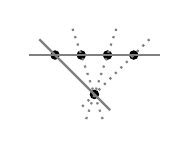
\begin{tikzpicture}
\filldraw[black] (0,0) circle (1.5pt);
\filldraw[black] (1/3,0) circle (1.5pt);
\filldraw[black] (2/3,0) circle (1.5pt);
\filldraw[black] (1,0) circle (1.5pt);
\filldraw[black] (1/2,-1/2) circle (1.5pt);
\draw[gray,thick] (-1/3,0) -- (4/3,0);
\draw[gray,thick] (-1/5,1/5) -- (1/2+1/5,-1/2-1/5);
\draw[gray,thick,dotted] (1/3-1/9,1/3) -- (1/2+1/9,-1/2-1/3);
\draw[gray,thick,dotted] (2/3+1/9,1/3) -- (1/2-1/9,-1/2-1/3);
\draw[gray,thick,dotted] (6/5,1/5) -- (1/2-1/5,-1/2-1/5);
\end{tikzpicture}
\end{minipage} \\

Then $f(1,0,0)=f(0,1,0)=f(0,0,1)=0$ implies $a=b=c=0$, so it remains to show $\left\{\begin{aligned}
dx_1y_1+ex_1z_1+fy_1z_1&=0 \\ dx_2y_2+ex_2z_2+fy_2z_2&=0
\end{aligned} \right.$ has only one solution $(d,e,f)$ up to scaling (we've seen that $(d,e,f)$ and $(\lambda d,\lambda e,\lambda f)$ define the same conic by (a)). By calculating relevant determinants, this is equivalent to $[x_1:y_1:z_1],[x_2:y_2:z_2]$ are not the same point, which is assumed.
\end{enumerate}
\end{enumerate}
\end{enumerate}
\end{exe}

\begin{coro}
\label{coro:affineintdim}
Let $V,W\in\A^n$ be irreducible and quasiprojective of dimensions $d,e$. Then either $V\cap W=\varnothing$ or every irreducible component of $V\cap W$ has dimension $\geq d+e-n$.
\end{coro}
\begin{proof}
Embed $\A^n\hookrightarrow\A^n\times\A^n$ via $x\mapsto (x,x)$. The image $\Delta$ is $V(x_1-y_1,\ldots,x_n-y_n)=\bigcap_{i=1}^n H_i$ where $H_i=V(x_i-y_i)$ is a hyperplane; in particular $\Delta$ is a closed subset. Then $V\cap W=\{x\in\A^n:x\in V,x\in W\}$ can be identified with
\[
(V\times W)\cap\Delta=\{(x,y)\in\A^n\times\A^n:x\in V,y\in W,x=y\}=(V\times W)\cap\bigcap_{i=1}^n H_i,
\]
where $\dim V\times W=\dim V+\dim W=d+e$ by \ref{lemma:dimofprodissumofdim}. The rest follows by induction and \ref{thm:dimofintwithhp}.
\end{proof}

\begin{thm}
Let $V,W\subset\p^n$ be irreducible and quasiprojective of dimensions $d,e$ with $d+e\geq n$. Then either $V\cap W=\varnothing$ or every irreducible component of $V\cap W$ has dimension $\geq d+e-n$. If $V,W$ are projective, $V\cap W\neq\varnothing$.
\end{thm}
\begin{proof}
By replacing $V,W$ by projective closure, we can assume they are projective. Consider $\widetilde V,\widetilde W\subset\A^{n+1}$ the projective cones of $V,W$. Then $\dim\widetilde V=d+1,\dim\widetilde W=e+1$ by \ref{coro:dimofconeis1greater}, so each irreducible component of $\widetilde V\cap\widetilde W$ has dimension $\geq d+1+e+1-(n+1)=d+e-n+1\geq 1$, in particular not empty. Since $\widetilde V\cap\widetilde W$ is the cone of $V\cap W$, it follows $V\cap W\neq\varnothing$, and dimension follows from \ref{coro:affineintdim} and again \ref{coro:dimofconeis1greater}.
\end{proof}

\begin{flushright}
\textit{Week 8, lecture 1, 24th February: correction of coursework 1, dimension continued}
\end{flushright}

\begin{enumerate}
\item You can omit $\{(0,0)\}$ since it's contained in the line $\{x=y\}$.
\item Note that we also need to consider the case $\Char =2$: for $V(f,g)$, if $\Char k=2$ then $\{(t,-t,-t^3)\}$ and $\{t,t,t^3\}$ are the same cubic, and similarly for $V(f,h)$, $i^2=-1=1$ so $i=1$ and the 4 parabolas are in fact the same one, and finally $V(f,g,h)$ is just 2 points.
\item Writing $\im\phi=V\left(y^p-x^q\right)$ is not entirely correct. One should take $d=\gcd(p,q)$, write $p=dp',\ q=dq'$ and $\im\phi=V\left(y^{p'}-x^{q'}\right)$. For the second part, again we need to consider other characteristics: $\zeta^p=\zeta^q=1$ can also happen if $\gcd(p,q)$ is some power of $\Char k$.
\item This is very similar to some of the exercises we've done in lecture before.
\item Explicitly, we have the projection map $\pi:V\dashrightarrow\p^2:[w:x:y:z]\mapsto[w:x:y]$ with inverse $\psi:\p^2\dashrightarrow V:[w:x:y]\mapsto [wy:xy:y^2:wx]$.
\end{enumerate}

We want to generalise \ref{thm:dimofintwithhp} by \textbf{Veronese embedding}. Let $d,n\in\Z^+$ and consider monomials of degree $d$ in $k[x_0,\ldots,x_n]$. In total there are $\binom{n+d}{d}$ of such monomials. Let $N=\binom{n+d}{d}-1$. Define the Veronese embedding
\[
\nu_{n,d}:\p^n\rightarrow\p^N:[x_0:\cdots:x_n]\mapsto \left[\text{all monomials of degree }d\text{ in }x_0,\ldots,x_n\right]
\]
this is regular since if $(x_0,\ldots,x_n)\neq (0,\ldots,0)$ then suppose $x_i\neq 0$ so $x_i^d\neq 0$.

For example,
\[
\nu_{2,2}:\p^2\rightarrow\p^5:[x_0:x_1:x_2]\mapsto [x_0^2:x_1^2:x_2^2:x_0x_1:x_1x_2:x_0x_2].
\]
We see that the Veronese embedding is an isomorphism on its image which is closed in $\p^N$ (in particular determined by homogeneous polynomials of degree $d$). Also, if we have $\widetilde V(f)\subset \p^n$ where $f$ is homogeneous of degree $d$, then write $f=\sum\alpha_\mu x_0^{\mu_0}\cdots x_n^{\mu_n}$, so that $\nu_{n,d}\left(\widetilde V(f)\right)=\nu_{n,d}(\p^n)\cap \widetilde V\left(\sum\alpha_mu x_\mu\right)$ where $\sum\alpha_mu x_\mu$ is now a linear polynomial, hence $\widetilde V\left(\sum\alpha_mu x_\mu\right)$ is some hyperplane in $\p^N$.
\begin{flushright}
\textit{Week 8, lecture 2, 27th February}
\end{flushright}

We therefore have a generalised \ref{thm:dimofintwithhp} which follows from \ref{thm:dimofintwithhp} itself:
\begin{thm}
\label{thm:gendimofintwithhp}
Let $V\subset\p^n$ be irreducible and quasiprojective and $H$ a hyperplane of $\p^n$ such that $V\not\subset H$. Then either $V\cap H=\varnothing$ or every irreducible component of $V\cap H$ has dimension $\dim V-1$. If $V$ is projective then $V\cap H\neq\varnothing$.
\end{thm}

\subsubsection{Topological definition}
\begin{lemma}
Let $V$ be irreducible and quasiprojective and $W$ be an irreducible and closed subset of $V$. Then $\dim W\leq\dim V$ with equality iff $V=W$.
\end{lemma}
\begin{proof}
For the first part:
\begin{itemize}
\item Geometric proof: restrict to affine open subset of $V$, i.e. assume $V$ is affine, and as usual replace $V,W$ by their projective closures, i.e. assume $V,W$ are projective. Then there is a finite-to-one, surjective map $V\rightarrow\p^n$ where $n=\dim V$. By iterating projections to hyperplane, there is a finite-to-one, surjective map $W\rightarrow\p^{n-r}$ for some $r\geq 0$. Hence $\dim W=n-r\leq n=\dim V$.
\item Algebraic proof: still assume $V$ is affine, then there is a surjective ring homomorphism $k[V]\rightarrow k[W]$ and in particular a surjective field homomorphism $k(V)\rightarrow k(W)$. Hence $k(W)\subset k(V)$ is a field extension, so transcendence degree of $k(W)$ is greater than or equal to that of $k(V)$, which implies the desired by the algebraic definition of dimension.
\end{itemize}
For the second part, write $V\subset\p^n$ is quasiprojective and $W\subsetneq V$. Then there is a homogeneous polynomial $f\in k[x_0,\ldots,x_n]$ such that $f$ vanishes on $W$ but not on $V$. Denote by $H$ the hyperplane defined by $f$. Then $V\not\subset H$ and $W\subset V\cap H$, so by \ref{thm:gendimofintwithhp} each irreducible component of $V\cap H$ has $\dim V-1$, so $\dim W\leq \dim V-1<\dim V$.
\end{proof}

\begin{thm}
Let $V$ be irreducible and quasiprojective. The dimension of $V$ is the maximal integer $d$ such that there is a chain of irreducible closed subsets $V=V_d\supsetneq V_{d-1}\supsetneq\cdots\supsetneq V_0\supsetneq\varnothing$.
\end{thm}
\begin{proof}
Take an irreducible component $V_d$ of $V$, find a hyperplane $H$ such that $V_d\not\subset H$, apply \ref{thm:gendimofintwithhp} and take $V_{d-1}$ to be $V_d\cap H$, and iterate this until $\dim V=0$ and label this $V_0$. At each step, $\dim V_i=\dim V_{i+1}-1$, hence $d=\dim V$. It also follows from previous lemma that there's no such sequence with $d>\dim V$.
\end{proof}

The theorem itself is not strong enough to be useful, i.e. even if we successfully write down such a sequence and we cannot insert other irreducible closed subsets into it, we still don't have a way to know its length is maximal. But we don't have to worry about this since we have Krull dimension (you know this from Atiyah's \textit{Commutative algebra}), and as long as the chain is \textit{maximal} in the sense that we cannot insert more, then it's \textit{maximal} in the sense that there's no other longer chain.

\subsubsection{Fibre theorem}
Let $f:V\rightarrow W$ be a regular map of quasiprojective varieties and $p\in W$ a point. Call the closed subset $f^{-1}(p)\subset V$ the \textit{fibre} of $f$ at $p$. Recall that $\dim V\times W=\dim V+\dim W$, and for projection $p_2:V\times W\rightarrow W$ and $p\in W$ we have $f^{-1}(p)=V\times \{p\}$, so its dimension is $\dim V=\dim V\times W-\dim W$. We want to do this in more generality.

(!) We assume that $f$ is dominant for dimension consistency (if we have $\{0\}\hookrightarrow\A^n$ then we would have that fibre of any point is dimension 0).

Also, consider $f:\A^3\rightarrow\A^2:(x,y,z)\mapsto(xy,xz)$. Over $p=(s,t)\neq (0,0)$ one has $f^{-1}(p)=\{(x,y,z):xy=s,xz=t\}$. By symmetry assume $s\neq 0$. Then $x,y\neq 0$ and $y=sx^{-1},z=tx^{-1}$, so $f^{-1}(p)=\{(x,sx^{-1},tx^{-1}):x\in k^\times\}\cong\A^1\backslash\{0\}$ which has dimension $1=\dim\A^3-\dim\A^2$. But $f^{-1}((0,0))=\{(x,y,z):xy=xz=0\}=V(x)\cup V(y,z)$ is not irreducible and its components have dimension 2 and 1.

\begin{thm}[Fibre dimension]
Let $V,W$ be irreducible and quasiprojective and $f:V\rightarrow W$ dominant and regular. Then
\begin{enumerate}
\item $\forall w\in W$, each irreducible component of $f^{-1}(w)$ has dimension at least $\dim V-\dim W$.
\item There is a nonempty open subset $U\subset W$ such that each irreducible component of $f^{-1}(w)$ has dimension exactly $\dim V-\dim W\ \forall w\in U$.
\end{enumerate}
\end{thm}

\begin{flushright}
\textit{Week 8, lecture 3, 28th February}
\end{flushright}

\begin{proof}
\begin{enumerate}
\item Cover $W$ with affine open subsets $U_i$ and $f^{-1}(U_i)$ with $U_{ij}'$. Then $f_{ij}:U_{ij}'\rightarrow U_i$ is dominant, so we can assume $V,W$ to be affine. Now $f$ corresponds to $f^\ast:k[W]\rightarrow k[V]$, which by \ref{defn:isoembdomin} is injective. Let $f_1,\ldots,f_n\in k[W]$ be a transcendence basis of $k(W)$ and consider $g_1,\ldots,g_m\in k[V]$ such that $f_1,\ldots,f_n,g_1,\ldots,g_m$ is a transcendence basis of $k(V)$. Then $\dim W=n$ and $\dim V=n+m$.

Recall Nullstellensatz and \ref{example:ringofregfunc} and see that a point $u\in W$ corresponds to a maximal ideal $\m_u\subsetneq k[W]\hookrightarrow k[V]$ and $k[f^{-1}(u)]=k[V]/\m_u$. Now $g_1,\ldots,g_m\in k[V]$ are algebraically independent over $k[W]$, hence gives $m$ algebraically independent elements of a prime ideal $I\subset k[V]/\m_u=k[f^{-1}(u)]$ over $k[W]/\m_u=k$, so every irreducible component of $f^{-1}(u)$ has degree at least $m=\dim V-\dim W$.
\item Consider $h_1,\ldots,h_r\in k[V]$ such that $f_1,\ldots,f_n,g_1,\ldots,g_m,h_1,\ldots,h_r$ generate $k[V]$. By construction $h_i$'s are algebraic in $f_1,\ldots,f_n,g_1,\ldots,g_m$, i.e. for each $h_i$ we can take $F_i\in k[f_1,\ldots,f_n,g_1,\ldots,g_m][x]$ such that $F_i(h_i)=0$. In particular, write $F_i(h_i)=c_dh_i^d+c_{d-1}h_i^{d-1}+\cdots+c_0$ where $c_j\in k[f_1,\ldots,f_n,g_1,\ldots,g_m]$ and $c_d\neq 0$. Consider $c_d\in k[g_1,\ldots,g_m][f_1,\ldots,f_n]$ and let $U_i=\{u\in W:c_d(f_1(u),\ldots,f_n(u))\neq 0\}$ and $U=\bigcap_{i=1}^rU_i$. Then $u\in U$ means $h_i$'s are algebraic over $g_1,\ldots,g_m$ in $k[f^{-1}(u)]$, so combining with part 1 we have that $g_1,\ldots,g_m$ is a transcendence basis of $k(V')$ where $V'$ is an irreducible component of $f^{-1}(u)$, i.e. every irreducible component of $f^{-1}(u)$ has dimension $m$. It just remains to see that $U$ is open since it's defined by the non-vanishing of a polynomial.
\end{enumerate}
\end{proof}

The theorem is useful when we know $\dim V$ or $\dim W$ but not the other, and we work out $\dim f^{-1}(w)$ for some $w\in W$ to get an inequality. In particular if some $\dim f^{-1}(w)=0$ then $\dim V-\dim W\leq 0$, i.e. $\dim V\leq \dim W$, but we know $\dim W\leq \dim V$ by the proof of part 1 of the theorem, so $\dim V=\dim W$.

\begin{example}
Consider $\varphi:\A^2\rightarrow\A^2:(x,y)\mapsto(x,xy)$ and the line $L_x=\{(x,y):y\in k\}$ where $x$ is fixed. If $x\neq 0$ then $\varphi:L_x\rightarrow L_x$ is an isomorphism; if $x=0$ then $\varphi$ maps the whole line $L_0$ to 0. This verifies the theorem: on the open set $\{(x,y)\in L_x:x\neq 0\}$ we then have $\dim\varphi^{-1}(x,y)=0=\dim\A^2-\dim\A^2$ (a single point), and $\dim\varphi^{-1}((0,0))=\dim L_0=1\geq 0$.
\end{example}

Another usage is a criteria for irreducibility. Note that if $f:V\rightarrow W$ is a dominant and regular map between quasiprojective varieties and $V$ is irreducible, then $W$ is irreducible; indeed, if $W=W_1\cup W_2$ then $V=f^{-1}(W_1)\cup f^{-1}(W_2)$, so WLOG $V=f^{-1}(W_1)$ and hence $W=W_1$. In general the converse (if $W$ is irreducible then $V$ is) is false but we can use the fibre theorem to impose some condition to have a partial converse.

\begin{prop}
\label{prop:fibVirrsamedimimpVirred}
Let $f:V\rightarrow W$ be surjective and suppose $V$ is projective, $W$ is irreducible, and fibres of $V$ are all irreducible of same dimension $d$. Then $V$ is irreducible.
\end{prop}
\begin{proof}
Let $V_1,\ldots,V_n$ be irreducible components of $V$. By \ref{thm:completeisprojective} $V$ is complete, so $f(V_i)$ is closed, and since $f$ is surjective, $W=\bigcup_{i=1}^nf(V_i)$. Since $W$ is irreducible, $W=f(V_i)$ for some $i$. Fix this $i$ and we have a surjective restriction $f_i:V_i\rightarrow W$. Let $U_i=V_i\backslash\bigcup_{j\neq i}V_j$. This is a nonempty and open subset of $V_i$, and also dense in $V_i$ since $V_i$ is irreducible. Then $f_i(U_i)$ is dense in $W$. Indeed, take any nonempty open subset $U\subset W$, then $f_i^{-1}(U\cap f_i(U_i))\supset f_i^{-1}(U)\cap U_i$ is nonempty since $U_i$ is dense, so $U\cap f_i(U_i)\neq\varnothing$. Hence $f_i$ is dominant.

Now let $w\in W$ and write $f^{-1}(w)=\bigcup_j f^{-1}(w)\cap V_j$. But we assumed fibres are irreducible, so $f^{-1}(w)\subset V_j$ for some $j$, and if $w\in f_i(U_i)$ then clearly $f^{-1}(w)\subset V_i$, so $f^{-1}(w)=f_i^{-1}(w)$ and by the fibre dimension theorem, $\dim V_i=\dim W+\dim f_i^{-1}(w)=\dim W+\dim f^{-1}(w)=\dim W+d$.

But by assumption, since $f$ is surjective (so in particular dominant), we also have $\dim V=\dim W+d$, hence $\dim V=\dim V_i$, which forces $V=V_i$.
\end{proof}

(!) We do need that $V$ is projective: if $V\subset\A^2$ is the union of the hyperbola $V(xy-1)$ and the origin, which is clearly reducible, then $V$ projects surjectively on $\A^1$ with each fibre a single point (hence in particular irreducible of same dimension).

\begin{flushright}
\textit{Week 9, lecture 1, 3rd March: problem class (sheet 5)}
\end{flushright}

\begin{exe}
\begin{enumerate}
\item Let $V\subset\p^n$ be a projective variety with all components of dimension $n-1$. Prove $V$ is a hypersurface.

\textit{Solution}. Write $V=V_1\cup\cdots\cup V_n$ where $V_i$'s are irreducible components of $V$ and by assumption $\dim V_i=n-1$. Consider a nontrivial homogeneous polynomial $g_i$ which vanishes on $V_i$. As $V_i$ is irreducible, each irreducible factor of $g_i$ vanishes on $V_i$. Let $f_i$ be a irreducible factor of $g_i$. Then $V_i\subset\widetilde V(f_i)\subset\p^n$ where $V(f_i)$ is a irreducible hypersurface of dimension $n-1$. But same is true for $V_i$, so $V_i=\widetilde V(f_i)$ and $V=\widetilde V(f_1\cdots f_n)$, a hypersurface.

This shows that $V\subset\p^n$ has irreducible components all of dimension $n-1$ iff $V$ is a hypersurface (the converse direction is trivial).

\item Let $H\subset\p^n$ be a hyperplane and $V\subset H$ a irreducible projective variety. Let $x\in\p^n\backslash H$ and $C=\bigcup_{p\in V}L_{xp}$. Prove that $C$ is projective, irreducible, and $\dim C=\dim V+1$.

\textit{Solution}. Choose coordinates such that
\[
H=\{[0:x_1:\cdots:x_n]:(x_1,\ldots,x_n)\in k^n\backslash\{0\}\}\qquad \text{and} \qquad x=[1:0:\cdots:0].
\]
Then $C=\{[s:tx_1:\cdots:tx_n]:[0:x_1:\cdots:x_n]\in V,\ s,t\in k^\times\}$. Let $f_1,\ldots,f_r\in k[x_1,\ldots,x_n]$ be homogeneous of the same degree such that $V=\{[0:x_1:\cdots:x_n]:f_i(x_1,\ldots,x_n)=0 \ \forall i=1,\ldots,r\}$. But then $C=\widetilde V\left(g_1,\ldots,g_r\right)$ where $g_i(x_0,\ldots,x_n)=f_i(x_1,\ldots,x_n)$, in particular $C$ is projective. Since $V$ is irreducible, $\sqrt{f_i}$'s are prime, so $\sqrt{g_i}$'s are prime, so $C$ is irreducible. Now note that $C\backslash\{x\}\cong V\times\A^1$, then $\dim C=\dim C\backslash\{x\}=\dim V+\dim\A^1=\dim V+1$.

\item Let $V_{n,d}$ be the vector space of homogeneous polynomials of degree $d$ in $k[x_0,\ldots,x_n]$ and $P_{n,d}$ be the projective space to $V_{n,d}$.
\begin{enumerate}
\item Show that for each $e:0\leq e\leq d$, multiplication of polynomials $V_{n,e}\times V_{n,d-e}\rightarrow V_{n,d}$ induces a regular map $\mu_{n,d,e}:P_{n,e}\times P_{n,d-e}\rightarrow P_{n,d}$.
\item By applying completeness to $\mu_{n,d,e}$, show that $P_{n,d,\irr}=\{[f]\in P_{n,d}:f\text{ is irreducible}\}$ is an open subset of $P_{n,d}$.
\item Let $n\geq 2$. Prove that $P_{n,d,\irr}\neq\varnothing$.
\item Prove that $P_{n,d,\rad}=\{[f]\in P_{n,d}:f\text{ generates a radical ideal}\}$ is an open subset of $P_{n,d}$.
\item Give an example of $f,g\in V_{n,d}$ with $[f],[g]\in P_{n,d}\backslash P_{n,d,\rad}$ such that $f$ is not a scalar multiple of $g$ but $f,g$ defines the same hypersurface in $\p^n$.
\end{enumerate}

\textit{Solution.} \begin{enumerate}
\item Note that $([f],[g])\mapsto [fg]$ is bilinear, so we only need to check multiplication of polynomials which are homogeneous of degree 1 in one variable, which is clear.
\item Note that $f$ is reducible iff it's in the image of $\mu_{n,d,e}$ for $1\leq e\leq d-1$, which is closed.
\item Note that $x_0^2-x_1x_2\in P_{2,2,\irr}$.

Generally, note that $\dim V_{n,d}=\binom{n+d}{d}$, so $\dim P_{n,d}=\binom{n+d}{d}-d$, and
\[
\dim P_{n,e}\times P_{n,d-e}=\binom{n+e}{e}+\binom{n+d-e}{d-e}-d<\binom{n+d}{d}+1-d,
\]
i.e. $\dim P_{n,d,\irr}>1$.
\item $f$ generates a radical ideal iff each of its irreducible factor appears only once, i.e. one cannot write $f=gh^r$ for $h\geq 2$. Now consider $a,b,r:ar+b=d$ with $r\geq 2$, then image of $\mu_{n,a,b,r}:P_{n,a}\times P_{n,b}\rightarrow P_{n,d}:([f],[g])\mapsto [f^2g]$ is closed, and $P_{n,d,\rad}$ is precisely the complement of its union over $a,b,r$.
\item $x_0^{d-1}x_1,\ x_0x_1^{d-1}$.
\end{enumerate}

\begin{flushright}
\textit{Week 9, lecture 2, 6th March}
\end{flushright}

\item Let $V\subset\p^n$ be an irreducible, projective variety of dimension $d$.
\begin{enumerate}
\item Let $\Sigma=\{(p,q,r)\in V\times V\times \p^n:p\neq q\text{ and }r\in L_{pq}\}$ and $\overline\Sigma$ be its Zariski closure. Suppose $\overline\Sigma$ is irreducible, and $\overline\Sigma\cap\{(p,q,r)\in V\times V\times \p^n:p\neq q\}=\Sigma$. Prove that projection $\pi_{1,2}:\overline\Sigma\rightarrow V\times V$ is surjective.
\item Show that $\dim\overline\Sigma\leq 2d+1$ by applying the fibre dimension theorem to $\pi_{1,2}:\overline\Sigma\rightarrow V\times V$.
\item Let\[
S=\bigcup_{\substack{(p,q)\in V\times V\\ p\neq q}}L_{pq}
\]
and denote by $\pi_3$ the projection $\overline\Sigma\rightarrow\p^n$ to the third factor. Prove that $\pi_3(\Sigma)=S$ and $S$ is contained in some closed subset of $\p^n$ of dimension at most $2d+1$.
\item Deduce that if $2d+1<n$ then there is a point $r\in\p^n$ such that every line through $r$ intersects $V$ in at most one point.
\end{enumerate}

\textit{Solution}. \begin{enumerate}
\item As $V$ is projective, $V\times V\times\p^n$ is projective, and since $\overline\Sigma\subset V\times V\times\p^n$ is closed, it is projective and in particular complete, so $\pi_{1,2}(\overline\Sigma)$ is closed in $V\times V$. But the image of $\pi_{1,2}:\Sigma\rightarrow V\times V$ is the dense open subset $\{(p,q)\in V\times V:p\neq q\}$, and clearly $\pi_{1,2}(\overline\Sigma)\supset\pi_{1,2}(\Sigma)$, so $\pi_{1,2}(\overline\Sigma)=V\times V$.
\item We know $\dim(V\times V)=2\dim V=2d$. To have the desired inequality using fibre dimension theorem, it suffices to show each irreducible component of a fibre has dimension at least 1. Let $(p,q)\in V\times V$ with $p\neq q$. Then $\pi_{1,2}^{-1}((p,q))=\{r\in\p^n:(p,q,r)\in\overline{\Sigma}\}=\{r\in\p^n:r\in L_{pq}\}=L_{pq}$ which has dimension 1.
\item $r\in\pi_3(\Sigma)\iff\exists p\neq q\in V:r\in L_{pq}\iff r\in S$. Now $S\subset\pi_3(\overline\Sigma)$, where $\pi_3(\overline\Sigma$ is closed (similar to in (a) that $\pi_{1,2}(\overline\Sigma)$ is closed). Now $\overline{\Sigma}$ is irreducible and by (b) has dimension at most $2d+1$, so its image has dimension at most $2d+1$ too.
\item By (c), the assumption means $S$ is contained in a closed subset of $\p^n$ of dimension $<n$, so $S\subsetneq\p^n$, hence $\exists r\in\p^n\backslash S$, i.e. $r$ is not in any line through two different points of $V$, i.e. any line through $r$ intersects $V$ in at most one point, exactly as desired.
\end{enumerate}
\end{enumerate}
\end{exe}

\subsection{Parameter spaces}
Let $B$ be a quasiprojective variety. A \textit{family of projective algebraic varieties} over $B$ is a Zariski-closed subset $\V\subset B\times\p^n$. For each $b\in B$, write $\V_b=\{x\in\p^n:(b,x)\in V\}$ and call this a fibre of $\V$. $B$ is then the \textit{base} or \textit{parameter space} of the family $\V$.

\begin{example}
In fact we've already seen some example. A hypersurface of degree $d$ in $\p^n$ is defined by a homogeneous polynomial of degree $d$ in $n$ variables. Denote by $V_{n,d}$ the vector space of homogeneous polynomials of degree $d$ in $k[x_0,\ldots,x_n]$ and let $P_{n,d}=V_{n,d}\backslash\{0\}/k^\times$. Let $\mathcal H=\{([f],x)\in P_{n,d}\times\p^n:f(x)=0)\}$. This is closed, so it's a family of projective algebraic varieties over $P_{n,d}$. Then a fibre is
\[
\mathcal H_{[f]}=\{x\in\p^n:([f],x)\in\mathcal H\}=\{x\in\p^n:f(x)=0)\}=\text{the hypersurface defined by }f
\]
(two different homogeneous polynomials differ by scaling define the same hypersurface).

Fix $x\in\p^n$ and write coordinates $x=[0:\cdots:0:1]$. Consider the set of hypersurfaces containing $x$: $\{[f]\in P_{n,d}:x\in\mathcal H_{[f]}\}$, which can be written as $\{[f]\in P_{n,d}:f_{0\cdots 0d}=0\}$ where $f_{i_0\cdots i_n}$ is the coefficients of $f\in V_{n,d}$ (with respect to the basis $x_0^{i_0}\cdots x_n^{i_n}$), hence the set itself is a hypersurface in $P_{n,d}$, in particular closed. One therefore sometimes says that the condition that ``the hypersurface $f$ defines contains a given point $x$'' is a \textit{closed condition} on $f$. Similarly, as we've seen in exercise 3 above, irreducibility and generating a radical ideal are \textit{open conditions}. In general it's more in our interest to study closed conditions since we can use the dimension theory we just developed on closed sets, while recall that if $U\subset V$ is open then $\dim U=\dim V$.

\subsubsection{Intersection of hypersurfaces}
Consider the intersection of $n+1$ hypersurfaces in $\p^n$. From our previous result on dimensions of intersections (\ref{thm:gendimofintwithhp}), generally if they are different hypersurfaces this intersection would be empty. For simplicity, suppose the $n+1$ hypersurfaces all have degree $d$. Consider the parameter space $(P_{n,d})^{n+1}$ and its subset
\[
S=\left\{([f_0],\ldots,[f_n])\in(P_{n,d})^{n+1}:\bigcap_{i=0}^n\mathcal H_{[f_i]}\neq\varnothing\right\}.
\]
Let
\[
\Sigma=\left\{([f_0],\ldots,[f_n],x)\in (P_{n,d})^{n+1}\times\p^n:x\in\mathcal H_{[f_0]} \ \forall i\right\}
\]
and consider the projection $\pi_1:\Sigma\rightarrow(P_{n,d})^{n+1}$. Note that
\[
\pi_1^{-1}(([f_0],\ldots,[f_n]))\cap\Sigma\neq\varnothing \iff ([f_0],\ldots,[f_n])\in S,
\]
i.e. $S=\pi_1(\Sigma)$, in particular $\pi_1:\Sigma\rightarrow S$ is surjective. Now together with the second projection $\Sigma\rightarrow\p^n$, we can use fibre dimension theorem to compute $\dim S$ to ``measure'' how far away the $n+1$ hypersurfaces are from general.
\end{example}

\begin{flushright}
\textit{Week 9, lecture 3, 7th March}
\end{flushright}

Let $x\in\p^n$, then its fibre is
\[
\pi_2^{-1}(x)=\{([f_0],\ldots,[f_n],x):x\in\mathcal H_{[f_i]} \ \forall i\}=\{([f_0],\ldots,[f_n],x):f_i(x)=0 \ \forall i\}\cong\left(\{[f]\in P_{n,d}:f(x)=0\}\right)^{n+1}
\]
since the $n+1$ polynomials are independent. As $x$ is fixed, $f$ is a homogeneous polynomial of degree 1 in its coefficients, so $\pi_2^{-1}(x)$ is a product of $n+1$ hypersurfaces in $P_{n,d}$, hence is irreducible of degree
\[
(n+1)(\dim P_{n,d}-1)=(n+1)\left(\binom{n+d}{d}-2\right).
\]
As $x$ is arbitrary, this means $\pi_2$ is surjective, and clearly $\p^n$ is irreducible  so by \ref{prop:fibVirrsamedimimpVirred} $\Sigma$ is irreducible. Hence by fibre dimension theorem (since all fibres have same dimension we can directly use the strong version),
\[
\dim\pi_2^{-1}(x)=(n+1)\left(\binom{n+d}{d}-2\right)=\dim\Sigma-\dim\p^n=\dim\Sigma-n,
\]
i.e.
\[
\dim\Sigma=(n+1)\left(\binom{n+d}{d}-2\right)+n=(n+1)\binom{n+d}{d}-n-2
\]

Now $S=\pi_1(\Sigma)$ and $\Sigma$ is irreducible imply $S$ is irreducible, so we can apply the fibre dimension theorem to $\pi_1$. Note that for a fixed $([f_0],\ldots,[f_n])\in S$, its fibre is
\[
\pi_1^{-1}([f_0],\ldots,[f_n])=\left\{([f_0],\ldots,[f_n],x):x\in\bigcap_{i=0}^n\mathcal H_{[f_i]}\right\}\cong\bigcap_{i=0}^n\mathcal H_{[f_i]}\subset\p^n
\]
So choose $f_0=x_1,\ f_1=x_1,\ f_2=x_2,\ldots,f_n=x_n$, then $\bigcap_{i=0}^n\mathcal H_{[f_i]}$ is $\{[1:0:\cdots:0]\}$, a point, hence has dimension 0. By the theorem we have $0\geq\dim\Sigma-\dim S$, but of course $\dim\Sigma\geq\dim S$ since $\pi_2$ is surjective, so $\dim S=\dim\Sigma=(n+1)\binom{n+d}{d}-n-2=\dim(P_{n,d})^{n+1}-1$, in particular $S$ is a hypersurface in $(P_{n,d})^{n+1}$, so there is a polynomial in coefficients of $f_0,\ldots,f_n$ which vanishes iff $\bigcap_{i=0}^n\mathcal H_{[f_i]}\neq\varnothing$. This is completely nontrivial without dimension theory!

\subsection{Tangent space and smoothness (mastery material)}
\subsubsection{Tangent spaces with coordinates}
Let $V\subset\A^n$ be an affine variety with $x\in V$ and $f\in k[x_1,\ldots,x_n]$. Define
\[
df_x:k^n\rightarrow k:(a_1,\ldots,a_n)\mapsto \sum_{i=1}^n a_i\left.\frac{\partial f}{\partial x_i}\right|_x.
\]

(!) Differentials are weird in characteristic $p$, for example $\frac{\partial x^p}{\partial x}=px^{p-1}=0$, in particular that differential of $f$ vanishes doesn't imply $f$ is constant.

\begin{defn}
The \textit{tangent space} of an affine variety $V$ at at point $x\in V$ is $T_xV=\bigcap_{f\in I(V)}\ker df_x\subset k^n$.
\end{defn}

(!) Polynomials that generate $I(V)$ are not necessarily those that define $V$. Take for example $V=V(x^2)\subset\A^1$, then $V=\{0\}$ and $dx^2_x=\frac{\partial x^2}{\partial x}=2x$, so $\ker dx^2_0=\{x\in k:2\cdot 0=0\}=k$, but
\[
T_0V=\ker dx_0=\left\{x\in k : dx=\frac{\partial x}{\partial x}=1=0\right\}=\varnothing
\]

\begin{example}
Consider the line $L=V(x)\subset\A^2$, then
\[
dx_x(a_1,a_2)=a_1\frac{\partial x}{\partial x}+a_2\frac{\partial x}{\partial y}=a_1,
\]
hence
\[
T_xL=\ker dx_x=\{(a_1,a_2)\in k^2:a_1=0\}=\la(0,1)\ra.
\]
\end{example}

\begin{example}
Let $g\in k[x]$ and consider the graph $\Gamma=\{(x,g(x)):x\in k\}=V(y-g(x))$. Now $y-g(x)$ is monic of degree 1, hence irreducible, so $I(\Gamma)=(y-g(x))$. Now
\[
d(y-g(x))_x=a_1\frac{\partial (y-g(x))}{\partial x}+a_2\frac{\partial (y-g(x))}{\partial y}=-a_1g'(x)+a_2,
\]
so
\[
T_x\Gamma=\ker d(y-g(x))_x=\left\{(a_1,a_2)\in k^2:a_2=a_1g'(x)\right\}=\la(1,g'(x))\ra.
\]
\end{example}

\begin{example}[Cuspidal cubic]
Let $V=V(y^2-x^3)\subset\A^2$. Clearly $y^2-x^3$ is irreducible so $I(V)=(y^2-x^3)$. We have
\[
d(y^2-x^3)_x(a_1,a_2)=a_1\frac{\partial (y^2-x^3)}{\partial x}+a_2\frac{\partial (y^2-x^3)}{\partial y}=-3a_1x^2+2a_2y,
\]
so
\[
T_xV=\ker d(y^2-x^3)_x=\left\{(a_1,a_2)\in k^2:2a_2y=3a_1x^2\right\},
\]
in particular for the cusp at the origin, $T_{(0,0)}V=k^2$ and for any other point it's a line, which is a nice way of saying that the tangent line at $(0,0)$ is undefined.
\end{example}

\begin{lemma}
Let $V\subset\A^m,\ W\subset\A^n$ be affine varieties and $\phi:V\rightarrow W$ regular. For any $x\in V$, $\phi$ induces a linear map $d\phi_x:T_xV\rightarrow T_{f(x)}W$.
\end{lemma}
\begin{proof}
Since $\phi$ is regular, write $\phi(x)=(f_1(x),\ldots,f_n(x))$ where $f_1,\ldots,f_n\in k[x_1,\ldots,x_m]$. Consider the matrix $\left(\frac{\partial f_i}{\partial x_j}\right)_{ij}$ which gives a linear map $d\phi:k^m\rightarrow k^n$. Now for any $g\in k[y_1,\ldots,y_n]$, chain rule says $\frac{\partial g(f_1,\ldots,f_n)}{\partial x_j}=\frac{\partial g}{\partial y_i}\frac{\partial f_i}{\partial x_j}$,
hence $d\phi$ maps $\ker dg_x$ to $\ker dg_{\varphi(x)}$, in particular maps $T_xV$ to $T_{f(x)}W$. This also does not depend on the choice of $f_i$'s.
\end{proof}

\begin{flushright}
\textit{Week 10, lecture 1, 10th March}
\end{flushright}

In particular, if $\phi:V\rightarrow W$ is an isomorphism, then $d\phi_x:T_xV\rightarrow T_{\phi(x)}W$ is an isomorphism too with inverse $d\phi^{-1}_{\phi(x)}:T_{\phi(x)}W\rightarrow T_xV$, so we can defined the tangent space for any quasiprojective variety.

\subsubsection{Singular points}
Intuitively, at ``smooth points'', $\dim V=\dim T_xV$. But we would have a problem if $V$ is reducible, so we want to define smoothness as a local property.

\begin{defn}
Let $V$ be a quasiprojective variety. The \textit{local dimension} of $V$ at $x$, denoted by $\dim_xV$, is the maximum of dimensions of irreducible components of $V$ containing $x$.
\end{defn}

\begin{defn}
Let $V$ be a quasiprojective variety and $x\in V$. We say $x$ is a \textit{singular point} of $V$ if $\dim T_xV\neq \dim_xV$. Otherwise $x$ is a \textit{smooth point} of $V$.
\end{defn}

If we write $V=\bigcap_{i}V_i$ where $V_i$'s are irreducible components and have $x\in V_i\backslash\bigcup_{j\neq i}V_j$ for some $i$, then by definition $\dim xV=\dim_xV_i$, so $V$ is singular at $x$ iff $V_i$ is singular at $x$. It's possible to prove that if $x\in V_i\cap V_j$ with $i\neq j$ then $V$ is singular at $x$, but this requires Nakayama's lemma which won't be covered in this course. We focus on the proof of the following theorem.

\begin{thm}
\label{thm:SingVisproperclosed}
Let $V$ be an irreducible quasiprojective variety. Then the set of singular points of $V$, denoted by $\Sing V$, is a proper closed subset of $V$.
\end{thm}

Suppose $V$ is an irreducible hypersurface $V=V(f)\subset\A^n$ where $f\in k[x_1,\ldots,x_n]$ generates $I(V)$ and is irreducible. Then $\dim_xV=\dim V=n-1 \ \forall x\in V$. Now for any $x\in V$, $T_xV=\ker df_x\subset k^n$ has two possibilities of dimensions: if $df_x$ is constantly 0 then $T_xV=k^n$ so $\dim T_xV=n$, or if it's not then $T_xV$ is a hypersurface in $k^n$ with $\dim T_xV=n-1$. Hence by definition, in the latter case $x$ is smooth and in the previous $x$ is singular. Hence
\[
\Sing V=V\left(f,\frac{\partial f}{\partial x_1},\ldots,\frac{\partial f}{\partial x_n}\right)\subset\A^n,
\]
in particular closed. Recall that $\frac{\partial f}{\partial x_i}=0 \ \forall i\centernot\implies f$ is constant in characteristic $p$. But we can prove that this problem only happen if the exponent is a multiple of $p$.

\begin{lemma}
Let $k$ be a field with $\Char k=p>0$ and $f\in k[x]$. Then
\[
\frac{\partial f}{\partial x}=0\iff f=\sum_{i=0}^d a_{ip}x^{ip}.
\]
\end{lemma}
\begin{proof}
The $\impliedby$ direction is trivial. Now write $f=\sum a_ix^i$ in its general form. Then
\[
\frac{\partial f}{\partial x}=\sum ia_ix^{i-1}=0\iff ia_i=0 \ \forall i\iff a_i=0 \ \forall i:p\nmid i\iff f=\sum_{i=0}^d a_{ip}x^{ip}.
\]
\end{proof}

\begin{prop}
\label{prop:SingHclosedprop}
If $V\subset\A^n$ is a nonempty hypersurface, then $\Sing V\subsetneq V$.
\end{prop}
\begin{proof}
Write $V=V(f)$ where $f$ generates $I(V)$. Suppose per contra $\Sing V=V$. Then
\[
V\left(f,\frac{\partial f}{\partial x_1},\ldots,\frac{\partial f}{\partial x_n}\right)=V(f),
\]
so $f\mid\frac{\partial f}{\partial x_i} \ \forall i$, but $\deg \frac{\partial f}{\partial x_i}<f$, so $\frac{\partial f}{\partial x_i}=0 \ \forall i$. If $\Char k=0$ then $f$ is constant, contradicting that $V$ is a hypersurface. If $\Char k=p>0$, then
\[
f=\sum a_{pi_1\cdots pi_n}x_1^{pi_1}\cdots x_n^{pi_n}=\sum \left(b_{i_1\cdots i_n}x_1^{i_1}\cdots x_n^{i_n}\right)^p=\left(\sum b_{i_1\cdots i_n}x_1^{i_1}\cdots x_n^{i_n}\right)^p,
\]
in particular $f$ is not irreducible, contradicting that $f$ generates $I(V)$.
\end{proof}
Hence we've proved \ref{thm:SingVisproperclosed} for the special case of hypersurfaces.

\begin{lemma}
\label{lemma:SigmadVisclosed}
Let $V$ be a quasiprojective variety. For any $d\in\Z$, the set $\Sigma_d(V)=\{x\in V:\dim T_xV>d\}$ is closed.
\end{lemma}
\begin{proof}
A subset is closed iff its intersection with an open cover is closed, so assume $V\subset\A^n$ is affine. Write $I(V)=(f_1,\ldots,f_m)$. Then for $x\in V$, $T_xV=\bigcap_{i=1}^m\ker d{f_i}_x$. Interpret this as the kernel of the $m\times n$ matrix $M_x=\left(\frac{\partial f_i}{\partial x_j}\right)_{ij}$. By the rank--nullity theorem, $\dim T_xV=\dim k^n-\rk M_x$, so
\[
\Sigma_d(V)=\{x\in V:n-d>\rk M_x\}=\{x\in V:\text{every }(n-d)\times (n-d)\text{ submatrix of }M_x\text{ has det }0\},
\]
hence $\Sigma_d(V)$ is defined by polynomials, i.e. closed.
\end{proof}

\begin{lemma}
\label{lemma:Vnsisdense}
Let $V$ be an irreducible quasiprojective variety. The set of smooth points of $V$, denoted by $V_\ns$, is dense in $V$.
\end{lemma}
\begin{proof}
Let $U\subset V$ be open and nonempty. We prove $U\cap V_{\ns}\neq\varnothing$. Since $V$ is irreducible, $U$ is irreducible, so by \ref{prop:irraffvarisbirtohypsurf}, $U$ is birational to a hypersurface $H$, hence some open subset $U'$ of $U$ is isomorphic to an open subset of $H$. Since $\Sing H$ is closed and proper subset of $H$ (\ref{prop:SingHclosedprop}), $H_\ns=H\backslash\Sing H$ is an nonempty open subset of $H$, but since $H$ is irreducible, $H_\ns$ is dense in $H$. So $H_\ns\cap U'\neq\varnothing$, i.e. $U'\cap V_\ns\neq\varnothing$, and in particular $U\cap V_\ns\neq\varnothing$.
\end{proof}

\begin{lemma}
\label{lemma:dimTxVgeqdimxV}
Let $V$ be an irreducible quasiprojective variety. For every $x\in V$, $\dim T_xV\geq\dim_xV$.
\end{lemma}
\begin{proof}
By definition, since $V$ is already irreducible, $\dim_xV=\dim V=:d$. To prove the lemma, it's equivalent to show $\Sigma_{d-1}(V)=V$. By \ref{lemma:SigmadVisclosed}, $\Sigma_{d-1}(V)$ is closed, and since $V_\ns=\{x\in V:\dim T_xV=d\}\subset\Sigma_{d-1}(V)$, it's also dense. The desired then follows immediately.
\end{proof}

Now it remains to put everything together.

\begin{proof}[Proof of \ref{thm:SingVisproperclosed}]
By definition and \ref{lemma:dimTxVgeqdimxV}, $\Sing V=\{x\in V:\dim T_xV>\dim xV=\dim V=:d\}=\Sigma_d$ which is closed by \ref{lemma:SigmadVisclosed} and proper by \ref{lemma:Vnsisdense}.
\end{proof}

\begin{exe}[sheet 6]
\begin{enumerate}
\item Suppose $\Char k\neq 2,3$. For $a\in k$, denote by $V_a$ the surface
\[
V(x^3+y^3+z^3-3a(x^2+y^2+z^2)-a^2).
\]
Suppose that this polynomial generates $I(V_a)$. Describe $\Sing V_a$.

\textit{Solution}. Denote the polynomial defining $V_a$ by $f_a$. Then
\[
\begin{aligned}
\Sing V_a&=V\left(f_a,\frac{\partial f_a}{\partial x},\frac{\partial f_a}{\partial y},\frac{\partial f_a}{\partial z}\right)=V\left(f_a,3x^2-6ax,3y^2-6ay,3z^2-6az\right)\\
&=V_a\cap\left\{(x,y,z):x=0\text{ or }2a,y=0\text{ or }2a,z=0\text{ or }2a\right\}
\end{aligned}
\]

\begin{flushright}
\textit{Week 10, lecture 2, 13th March: problem class (sheet 6 continued)}
\end{flushright}

Now if $a=0$ then $\Sing V_a=\{(0,0,0)\}.$ If $a\neq 0$, consider a point $(x,y,z)$ where $n$ of its coordinates are equal to $2a$ and $3-n$ coordinates equal to 0. Then
\[
f_a(x,y,z)=n((2a)^3-3a(2a)^2)-a^2=-a^2(1+4na)=0\iff a=\frac{-1}{4n}.
\]

\item Let $V\subset\A^n,\ W\subset\A^m$ be affine and consider $v\in V,\ w\in W$. Prove that $V\times W$ is smooth at $(v,w)$ iff $V$ is smooth at $v$ and $W$ is smooth at $w$.

\textit{Solution}. Consider the irreducible components $V_i$ of $V$ and $W_j$ of $W$. Then
\[
V\times W=\left(\bigcup_i V_i\right)\times \left(\bigcup_j W_j\right)=\bigcup_{i,j}V_i\times W_j
\]
is the irreducible decomposition of $V\times W$. Then
\[
\begin{aligned}
\dim_{(v,w)}V\times W&=\max_{i,j:(v,w)\in V_i\times W_j}\dim V_i\times W_j=\max_{i,j:v\in V_i,w\in W_j} \left(\dim V_i+\dim W_j\right)\\
&=\max_{i:v\in V_i}\dim V_i+\max_{j:w\in W_j}\dim W_j=\dim_vV+\dim_wW.
\end{aligned}
\]
Now it suffices to prove $\dim T_{(v,w)}V\times W=\dim T_vV+\dim T_wW$, since then by definition $(v,w)$ is a smooth point of $V\times W$ iff $\dim T_{(v,w)}V\times W=\dim T_vV+\dim T_wW=0$. Consider $f_1,\ldots,f_t$ generating $I(V)\subset k[x_1,\ldots,x_n]$ and $g_1,\ldots,g_s$ generating $I(W)\subset k[y_1,\ldots,y_m]$. Then $\overline{f_1},\ldots,\overline{f_r},\overline{g_1},\ldots,\overline{g_s}$ where $\overline{f_i}(x_1,\ldots,x_n,y_1,\ldots,y_m)=f_i(x_1,\ldots,x_n)$ and $\overline{g_i}(x_1,\ldots,x_n,y_1,\ldots,y_m)=g_i(y_1,\ldots,y_m)$ generate $I(V\times W)$. Then $d\left(\overline{f_i}\right)_{(v,w)}:k^n\times k^m\rightarrow k:(a,b)\mapsto d(f_i)_V(a)$, so $\ker d\left(\overline{f_i}\right)_{(v,w)}=\ker d(f_i)_v\times k^m$. Similarly $\ker d\left(\overline{g_i}\right)_{(v,w)}=k^n\times\ker d(g_i)_w$. Hence
\[
\begin{aligned}
T_{(v,w)}V\times W&=\bigcap_{i=1}^r \ker d\left(\overline{f_i}\right)_{(v,w)}\cap \bigcap_{j=1}^s \ker d\left(\overline{g_j}\right)_{(v,w)} \\
&=\bigcap_{i=1}^r \left(\ker d(f_i)_v\times k^m\right)\cap \bigcap_{i=1}^s \left(k^n\times \ker d(g_j)_w\right) \\
&=\left(T_vV\times k^m\right)\cap\left(k^n\times T_wW\right)=T_vV\times T_wW,
\end{aligned}
\]
as desired.

\item Let $V\subset\A^n$ be an affine variety with irreducible components $V_1,V_2$. Consider $x\in V_1\cap V_2$. Prove that $TxV_1+T_xV_2\subset T_xV$.

\textit{Solution}. We have $V_1\subset V\implies I(V)\subset I(V_1)$. Let $a\in T_xV_1$ and write $TxV_1=\ker df_x$. Then $f\in I(V)\subset I(V_1)$, so $a\in T_xV$, i.e. $T_xV_1\subset T_xV$. Similarly $T_xV_2\subset T_xV$, thus $T_xV_1+T_xV_2\subset T_xV$.

Consider $V(y(y-x^2))=V(y)\cup V(y-x^2)=:V_1\cup V_2$ (union of $x$-axis and the parabola $y=x^2$) and let $x=(0,0)$. Then $T_xV_1=T_xV_2=x$-axis, so $T_xV_1+T_xV_2=x$-axis. But
\[
T_xV=\ker d(y(y-x^2))_x=\left\{(a_1,a_2)\in k^2:a_1(-2xy)+a_2(2y-x^2)=0\text{ where }x=y=0\right\}=k^2,
\]
so $T_xV_1+T_xV_2\subsetneq T_xV$.

\item Let $f$ be a nonzero polynomial in $k[x_1,\ldots,x_n]$ with no repeated factors, and $V\subset\A^n$ be the hypersurface defined by $f$. In particular $f$ generates $I(V)$.
\begin{enumerate}
\item Let $x\in V$ and $u\in k^n$. Prove that $f(x+Tu)\in k[T]$ has a repeated root at $T=0$ iff $u\in T_xV$.
\end{enumerate}

\textit{Solution}. We have
\[
\begin{aligned}
f(x+Tu)&=f(x)+T\sum_{i=1}^n u_i\left.\frac{\partial f}{\partial x_n}\right|_x+T^2 g(T)\in k[x] \\
&=f(x)+df_x(u)T+g(T)T^2\in k[T]
\end{aligned}
\]
and since $x\in V$, $f(x)=0$, so the order of root $T=0$ of $f(x+Tu)$ is 2 iff $df_x(u)=0$, i.e. $u\in\ker df_x=T_xV$.
\end{enumerate}
\end{exe}

\begin{flushright}
\textit{Week 10, lecture 3, 14th March}
\end{flushright}

\begin{flushright}
\textit{Week 11, lecture 1, 17th March}
\end{flushright}

The last two lectures went through the 2024 paper.

\end{document}
